\documentclass{article}


% if you need to pass options to natbib, use, e.g.:
%     \PassOptionsToPackage{numbers, compress}{natbib}
% before loading neurips_2022


% ready for submission
\usepackage{appendix}


% to compile a preprint version, e.g., for submission to arXiv, add add the
% [preprint] option:
%     \usepackage[preprint]{neurips_2022}


% to compile a camera-ready version, add the [final] option, e.g.:
%     \usepackage[final]{neurips_2022}


% to avoid loading the natbib package, add option nonatbib:
%    \usepackage[nonatbib]{neurips_2022}

% Use the postscript times font!
\usepackage{times}
\usepackage{soul}
\usepackage{url}
\usepackage[hidelinks]{hyperref}
\usepackage[utf8]{inputenc}
\usepackage[small]{caption}
\usepackage{graphicx}
\usepackage{amsmath}
\usepackage{amsthm}
\usepackage{amssymb,amsfonts}
\usepackage{booktabs}
\usepackage{algorithm}
\usepackage{algorithmic}
\usepackage{color}
\usepackage{subcaption}
\usepackage{enumitem}
\usepackage{pifont}
\usepackage{mathtools}
\usepackage{arydshln}
\usepackage{multirow}
% \usepackage{subfigure}
% \usepackage{array}
\urlstyle{same}

\newcommand{\modelParamter}{\omega}
\newcommand{\horizon}{T_{H}}
\newcommand{\datapoint}{x}
\newcommand{\condition}{z_{E}}
\newcommand{\state}{s}
\newcommand{\observation}{o}
\newcommand{\action}{a}
\newcommand{\transition}{t}
\newcommand{\reward}{r}
\newcommand{\agentIndex}{k}
\newcommand{\gameIndex}{j}
\newcommand{\quantielIndex}{i}
\newcommand{\dataset}{\mathcal{D}}
\newcommand{\expect}{\mathbb{E}}
\newcommand{\feature}{e}
\newcommand{\confidence}{c}
\newcommand{\error}{\epsilon}
\newcommand{\impact}{\phi}
\newcommand{\playerId}{l}
\newcommand{\constant}{C}
\newcommand{\splitnum}{m}
\newcommand{\sys}{RiGIM}
\newcommand{\bin}{B}
\newcommand{\goal}{g}
\newcommand{\system}{\sys\;}
\newtheorem{example}{Example}
\newtheorem{proposition}{Proposition}
\DeclareMathOperator*{\argmax}{argmax}

\title{Appendix}

% Single author syntax
\author{
}


\begin{document}

\maketitle

\appendix

\section{Implementation Details}
\renewcommand{\thetable}{A.\arabic{table}}
\renewcommand\thefigure{\thesection.\arabic{figure}}
\setcounter{table}{0}
\subsection{The Sports Dataset}

In this paper, we use an ice hockey and a soccer dataset. Table~\ref{table:feature-of-dataset} shows a complete list of features of these datasets. The dataset records the movements of each player in professional games. The data sources are game logs and broadcast videos, which are public resources. Personal information of these players, including age, gender, and physical conditions, has not been applied or discussed in this paper.

\begin{table}[htbp]
\begin{center}
\caption{The complete list of game features for the ice hockey dataset and the soccer dataset. 
% ES, SH and PP respectively denote Even Strength, Shorted Handed and Power Play. 
The table utilizes adjusted spatial coordinates where negative numbers denote the defensive zone of the acting player and positive numbers denote the offensive zone. 
% Adjusted X-coordinates run from -100 to +100 and Adjusted Y-coordinates from 42.5 to -42.5, where the origin is at the ice center. 
}
\label{table:feature-of-dataset}
\begin{tabular}{c|c|c|c}
\toprule
Type & Name & Range \\ \hline\hline
\multirow{12}{*}{\begin{tabular}[c]{@{}c@{}}Ice \\ Hockey\end{tabular}} & \multirow{5}{*}{\begin{tabular}[c]{@{}c@{}}Spatial \\ Features\end{tabular}} & X Coordinate of Puck & {[}-100, 100{]} \\
 & & Y Coordinate of Puck & {[}-42.5, 42.5{]} \\
 & & Velocity of Puck & $(-\infty,+\infty)$ \\
 & & Angle between & \multirow{2}{*}{\begin{tabular}[c]{@{}c@{}}[$-3.14$, $3.14$] \end{tabular}}\\ 
 & & the puck and the goal & \\\cline{2-4}
& \multirow{2}{*}{\begin{tabular}[c]{@{}c@{}}Temporal \\ Features\end{tabular}} & Game Time Left & {[}0, 3,600{]} \\
&  & Event Duration & (0, $+\infty$) \\ \cline{2-4}
& \multirow{5}{*}{\begin{tabular}[c]{@{}c@{}} In-Game \\ Features\end{tabular}} & Score Differential & $(-\infty,+\infty)$ \\
&  & \multirow{2}{*}{\begin{tabular}[c]{@{}c@{}} Manpower \\ Situation \end{tabular}} & \multirow{2}{*}{\begin{tabular}[c]{@{}c@{}}\{Even Strength, Shorted \\ Handed, Power Play\} \end{tabular}}\\
&  &  &  \\
&  & Home or Away Team & \{Home, Away\} \\
&  & Action Outcome & \{successful, failure\} \\ \hline\hline
Soccer  & \multirow{5}{*}{\begin{tabular}[c]{@{}c@{}}Spatial \\ Features\end{tabular}} & X Coordinate of ball & {[}0, 100{]} \\
 & & Y Coordinate of ball & {[}0, 100{]} \\
 & & Velocity of ball & $(-\infty,+\infty)$ \\
 & & Angle between & \multirow{2}{*}{\begin{tabular}[c]{@{}c@{}}[$-3.14$, $3.14$] \end{tabular}}\\ 
 & & the ball and the goal & \\\cline{2-4}
& \multirow{2}{*}{\begin{tabular}[c]{@{}c@{}}Temporal \\ Features\end{tabular}} & Game Time Remaining & {[}0, 100{]} \\
&  & Event Duration & (0, $+\infty$) \\ \cline{2-4}
& \multirow{5}{*}{\begin{tabular}[c]{@{}c@{}} In-Game \\ Features\end{tabular}} & Goal Differential & $(-\infty,+\infty)$ \\
&  & Manpower Situation  & [-5, 5]  \\
&  & Home or Away Team & \{Home, Away\} \\
% \multirow{2}{*}{\begin{tabular}[c]{@{}c@{}}Action\\ Type\end{tabular}} & Action Name & One-hot-vector \\
&  & Action Outcome & \{successful, failure\} \\ \hline\hline
\end{tabular}
\end{center}
\end{table}

\paragraph{Ice Hockey Dataset} In this paper, we use a play-by-play dataset constructed by Sportlogiq~\footnote{\url{https://sportlogiq.com}}. They capture the information of an on-puck player (player possessing the puck) from broadcast videos with computer vision techniques. In the experiments, we split the games in this dataset into training, testing, and validation datasets according to game dates, so the training dataset contains 956 games (from October 3rd, 2018 to February 24th, 2019), and the validation dataset contains 119 games (from February 24th, 2019 to March 12th, 2019), and the testing dataset contains 121 games (from March 12th, 2019 to April 6th, 2019).

\paragraph{Soccer Dataset} In this paper, we utilize the F24 play-by-play soccer game dataset provided by Opta\footnote{https://www.optasports.com/}. The dataset records the play-by-play information of game events and player actions for the entire 2017-2018 game season from multiple soccer leagues, including English Premier League, Dutch Eredivisie, EFL Championship, Italian Serie A, German Bundesliga, Spanish La Liga,  French Ligue 1 and German Bundesliga Zwei.

% \subsection{Model Implementation Details}

\subsection{Hyper-Parameters}
\begin{table}[htbp]
\centering
\caption{The Architecture of the main components in our model.}\label{table:model-architecture}
\begin{tabular}{c|c|c}
\hline
Model & Network Component & Hidden Dimensions \\ \hline
\multirow{6}{*}{Feature extractor} & Residual Layer & 128 \\
 & Leaky Rectified Linear Unit & N/A \\
 & Spectral Normalization & N/A \\
 & Residual Layer & 128 \\
 & Leaky Rectified Linear Unit & N/A \\
 & Spectral Normalization & N/A \\ \hline
 \multirow{6}{*}{Spline DRQN} & LSTM Layer & 128 \\
 & Fully Connect Layer & 128 \\
 & Rectified Linear Unit & N/A \\
 & Fully Connect Layer & 128 \\
 & Rectified Linear Unit & N/A \\
 & Spline function & N/A \\ \bottomrule
 \multirow{6}{*}{{\begin{tabular}[c]{@{}c@{}}A CNF Block \\ (i.e., MADE Layer~\cite{Germain2015made}\end{tabular}}} & Masked Linear Layer & 180 \\
 & Rectified Linear Unit & N/A \\
 & Masked Linear Layer & 180 \\
 & Batch Normalization & N/A \\
 & Reverse Layer & N/A \\ \bottomrule
\end{tabular}
% \begin{minipage}[t]{0.3\textwidth}
% \resizebox{1\textwidth}{!}{
% \begin{tabular}{cc}
% \toprule
% Network Component & Size \\ \hline
% Residual Layer & 128 \\
% Leaky Rectified Linear Unit & N/A \\
% Spectral Normalization & N/A \\
% Residual Layer & 128 \\
% Leaky Rectified Linear Unit & N/A \\
% Spectral Normalization & N/A \\ \bottomrule
% \end{tabular}
% }
% \end{minipage}
% % \begin{minipage}[0.5\textwidth]
% % \caption{The Feature Extractor}
% % \label{table:feature-extractor}
% \begin{minipage}[t]{0.3\textwidth}
% \resizebox{1\textwidth}{!}{
% \begin{tabular}{cc}
% \toprule
% Network Component & Size \\ \hline
% Fully Connect Layer & 128 \\
% Rectified Linear Unit & N/A \\
% Fully Connect Layer & 128 \\
% Rectified Linear Unit & N/A \\
% Spline Computation & N/A \\ \bottomrule
% \end{tabular}
% }
% \end{minipage}
% \begin{minipage}[t]{0.3\textwidth}
% \resizebox{1\textwidth}{!}{
% \begin{tabular}{cc}
% \toprule
% Network Component & Size \\ \hline
% Fully Connect Layer & 128 \\
% Rectified Linear Unit & N/A \\
% Fully Connect Layer & 128 \\
% Rectified Linear Unit & N/A \\
% Spline Computation & N/A \\ \bottomrule
% \end{tabular}
% }
% \end{minipage}
\end{table}

We introduce the hyper-parameters for implementing our distributional RL and FS-CNF models. Table~\ref{table:model-architecture} shows the model architecture.

\paragraph{Distributional RL model.} We set the quantile number $N$ to 64 and set the size of hidden layers (in both LSTM and Resnet) to be 128. The max trace length of LMST is set to 10, and the batch size is set to 64. The discount factor is set to 1, and the learning rate is set to 0.0005. The $\eta$ is set to 1.

\paragraph{FS-CNF.} The feature extractor is implemented by Residual layers and Spectral Normalization. To build CNF, we stack 5 layers of CNF blocks. Each block contains a MADE layer~\cite{Germain2015made}, a batch normalization layer, and a reverse layer by following the structure in ~\cite{Papamakarios2017MAF}. The size of a hidden layer is set to 180, and the learning rate is set to 0.0001.
% \begin{table}[htbp]
%     \centering
%     \begin{tabular}{c|c}
%     \toprule
%         Parameter Names &  Value \\ \hline
%         Agent Number $\MakeUppercase{\agentIndex}$ & 3 \\
%         Quantile Number $N$ & 64 \\
        
%         Hidden Parameters & 256 \\
        
%     \bottomrule
%     \end{tabular}
%     \caption{Caption}
%     \label{tab:my_label}
% \end{table}

\subsection{Gaussian Discriminant Analytic Model}
We introduce the implementation of our Gaussian Discriminant Analysis
(GDA) in our baselines. GDA is a Gaussian mixture model that builds a single Gaussian for each class $q(\feature|\Tilde{z}_{\splitnum})$ where 1) the class label $\Tilde{z}_{\splitnum}$ is constructed by dividing the expected returns $\expect(Z(\state,\action))\in[0,1]$ into $\splitnum$ classes $\{\Tilde{z}_{1},\dots,\Tilde{z}_{\MakeUppercase{\splitnum}}\}$. 2) we estimate the density for latent features $\feature$ instead of raw inputs $(\state,\action)$ since building GDA on spatial-temporal raw features is difficult and the higher-level latent features learned by neural networks can alleviate this difficulty~\cite{Mukhoti2021Uncertainty}. In order for $q(\feature|\Tilde{z}_{\splitnum})$ to capture the input density, the distance between data points in latent space must accurately reflect their distance in input space~\cite{Liu2020Uncertainty}. However, during learning, feature extractors might map the features of OoD inputs to InD regions in the latent space (i.e., Feature Collapse~\cite{Amersfoort2020Uncertainty} ). To fix this issue, we utilize a bi-Lipschitz constraint for the feature extractor $f(\datapoint;\modelParamter_{\mathcal{\MakeUppercase{\feature}}})$:
% \vspace{-0.15in}
\begin{align}
    & \forall{\datapoint_{1},\datapoint_{2}}\in\dataset \text{ and } \datapoint:=(\state,\action),\\
    & K_{1}\|\datapoint_{1}-\datapoint_{2}\|_{I}\leq\|f(\datapoint_{1};\modelParamter_{\mathcal{\MakeUppercase{\feature}}})-f(\datapoint_{2};\modelParamter_{\mathcal{\MakeUppercase{\feature}}})\|_{F}\leq K_{2}\|\datapoint_{1}-\datapoint_{2}\|_{I}\nonumber
\end{align}
where $\|\cdot\|_{I}$ and $\|\cdot\|_{F}$ denote metrics in the input and feature space
respectively, and $K1$ and $K2$ denote the lower and upper Lipschitz constants~\cite{Rosca2020smoothness}. The lower Lipschitz bound ensures sensitivity to distances in the input space, and the upper Lipschitz bound ensures smoothness in the features, preventing them from becoming too sensitive to input variations and leading to poor
generalisation and loss of robustness. We follow \cite{Liu2020Uncertainty} to ensure the bi-Lipschitzness in the feature extractor $f(\cdot;\modelParamter_{\mathcal{\MakeUppercase{\feature}}})$ by implementing it with residual connections together with spectral normalisation.

\subsection{Computation Resource and Running Time}
We run the experiment on a cluster operated by the Slurm workload manager. The cluster has multiple kinds of GPUs, including Tesla T4 with 16 GB memory, Tesla P100 with 12 GB memory, and RTX 6000 with 24 GB memory. 
Our program can be handled by the GPU with 12 GB of memory. We apply 24 GB of main memory for training the distributional RL and the FS-CNF models. The number of running nodes is 1, and the number of CPUs requested per task is 8. Given the aforementioned resources, the distributional RL program uses around 12 GPU hours to finish the training of 1 random seed for the ice-hockey dataset and 16 GPU hours for the soccer dataset (since the size of the soccer dataset is larger). 
Based on the well-trained distributional RL program, FS-CNF takes around 8 GPU hours 
to run the ice-hockey dataset and 10 GPU hours to run the soccer dataset. 

\paragraph{Computational Complexity.} Table~\ref{table:model-architecture} illustrates the structure of our model. \system is based on the mini-batch gradient descent. Let $B$ be the batch size, $M$ be the total number of data points, $N$ be the number of quantiles, $H$ be the size of hidden layers, $I$ be the input size, $T$ be maximum trace length of LSTM, $L$ be the number of layers in CNF and $K$ be the number of autoregressive layers in CNF.
The computational complexities of a forward pass of Resnet, LSTM, SPL-DQN and FS-CNF are $O(I^2+I)$, $O[T(IH+ I^2+I)]$, $O(H^2+NH^2)$~\cite{luo2022distributional} and $O[KIH+K(L-1)H^2]$~\cite{Papamakarios2017MAF} respectively. It requires $M/B$ passes to finish one round of training.
\paragraph{Memory Complexity.} Following the similar notation, the memory complexity of \system is $O[2I^{2}+4IH+(N+1)H^2+3KIH+K(L-1)H]$. This complexity is based on the size of parameters in our model. In practice, we also need to consider the influence of batch size.


\section{Proof}
% \subsection{Proposition 1.}
Let's assume we have vector valued random variables $\boldsymbol{Z}$, $\boldsymbol{\MakeUppercase{\reward}}$ with distribution space $ \mathcal{P}(\mathbb{R})^{|\MakeUppercase{\state}||\MakeUppercase{\action}|}$, so
% and we have a probability transition matrix $\boldsymbol{P}^{\pi}$ on state-action pairs induced by a stationary policy $\pi$:

\begin{align*}
    H(\boldsymbol{Z})& \stackrel{\mathclap{\normalfont\mbox{(a)}}}{=}H[(I-\gamma \boldsymbol{P}^{\pi})^{-1}\boldsymbol{\MakeUppercase{\reward}}]\\
    & \stackrel{\mathclap{\normalfont\mbox{(b)}}}{=}\log|\text{det}[(I-\gamma \boldsymbol{P}^{\pi})^{-1}]|+H[\boldsymbol{\MakeUppercase{\reward}}] \\
    & \stackrel{\mathclap{\normalfont\mbox{(c)}}}{=}\log|\text{det}[\frac{\mathbf{d}^{\pi}}{1-\gamma}]|+H[\boldsymbol{\MakeUppercase{\reward}}]\\
    & \stackrel{\mathclap{\normalfont\mbox{(d)}}}{=}-|A||S|\log(1-\gamma)+\log|\text{det}[\mathbf{d}^{\pi}]|+H[\boldsymbol{\MakeUppercase{\reward}}]
\end{align*}

\begin{itemize}
    \item (a) holds by following the Bellman consistency $\boldsymbol{Z}^{\pi}=\boldsymbol{\MakeUppercase{\reward}}+\gamma \boldsymbol{P}^{\pi} \boldsymbol{Z}^{\pi}$. To see that the $(I-\gamma \boldsymbol{P}^{\pi})$ is invertible, it suffices to show that for any non-zero vector $\boldsymbol{x}\in \mathbb{R}^{|\MakeUppercase{\state}|\times|\MakeUppercase{\action}|}$:
    \begin{align*}
        \|(I-\gamma \boldsymbol{P}^{\pi})\boldsymbol{x}\|_{\infty}&=\|\boldsymbol{x}-\gamma \boldsymbol{P}^{\pi}\boldsymbol{x}\|_{\infty}\\
        & \geq \|\boldsymbol{x}\|_{\infty}-\gamma \|\boldsymbol{P}^{\pi}\boldsymbol{x}\|_{\infty}\\
        & \geq \|\boldsymbol{x}\|_{\infty}-\gamma \|\boldsymbol{x}\|_{\infty}\\
        & = (1-\gamma)\|\boldsymbol{x}\|_{\infty}\\
        & \geq 0
    \end{align*}
    which implies $I-\gamma \boldsymbol{P}^{\pi}$ is full rank.
    \item (b) holds by following the differential entropy proprieties and the fact that $(I-\gamma \boldsymbol{P}^{\pi})$ is invertible.
    \item (c) holds by defining $\mathbf{d}^{\pi}=(1-\gamma)(I-\gamma \boldsymbol{P}^{\pi})^{-1}$. Here, we would like to show that $\mathbf{d}^{\pi}\in[0,1]^{|\MakeUppercase{\state}||\MakeUppercase{\action}|\times|\MakeUppercase{\state}||\MakeUppercase{\action}|}$ is the induced matrix for distributions over state-action tuples by following policy $\pi$. In other words, the $(\state,\action)^{th}$ row of $\mathbf{d}^{\pi}$ is an induced distribution over states and actions when following $\pi$ after starting with $\state_{0} = \state$ and $\action_{0} = a\action$. This follows from its definition: 
    \begin{align}
        \mathbf{d}^{\pi} & = (1-\gamma) \sum_{t=1}^{\infty}(\gamma\boldsymbol{P}^{\pi})^{t}\\
        & = \frac{(1-\gamma)[1-(\gamma\boldsymbol{P}^{\pi})^{\infty}]}{1-(\gamma\boldsymbol{P}^{\pi})} \\
        & = \frac{(1-\gamma)}{1-(\gamma\boldsymbol{P}^{\pi})}
    \end{align}

\end{itemize}


\section{Complementary Results}
\renewcommand{\thetable}{C.\arabic{table}}
\setcounter{table}{0}
\begin{table*}[htbp]
    \centering
    \resizebox{1\textwidth}{!}{
    \begin{tabular}{ccccccc}
    \toprule
         Methods & Assist & Goal & GWG & OTG & SHG & PPG \\\hline
         $+/-$ & 0.181  $\pm$  0 & 0.189  $\pm$  0 & 0.187  $\pm$  0 & 0.028  $\pm$  0 & 0.071  $\pm$  0 & -0.047  $\pm$  0 \\
         $EG$ & 0.239  $\pm$  0 & 0.303  $\pm$  0 & 0.264  $\pm$  0 & 0.130  $\pm$  0 & -0.053  $\pm$  0 & 184  $\pm$  0 \\
         $SI$ & 0.237  $\pm$  0 & 0.596  $\pm$  0 & 0.409  $\pm$  0 & 0.123  $\pm$  0 & 0.095  $\pm$  0 & 0.361  $\pm$  0 \\
         VAEP & 0.238  $\pm$  0.017& 0.454  $\pm$  0.013& 0.225  $\pm$  0.009& 0.06  $\pm$  0.005& 0.053  $\pm$  0.006& 0.315  $\pm$  0.004 \\
         T0-GIM & 0.397 $\pm$ 0.014 & 0.394 $\pm$ 0.016 & 0.139 $\pm$ 0.009 & 0.16 $\pm$ 0.006 & 0.151 $\pm$ 0.008 & 0.223 $\pm$ 0.021 \\
         GIM  & 0.456 $\pm$ 0.029 & 0.408 $\pm$ 0.029 & 0.167 $\pm$ 0.017 & 0.158 $\pm$ 0.007 & 0.134 $\pm$ 0.018 & 0.248 $\pm$ 0.014 \\
         Na-\sys$({0.5})$ & 0.593 $\pm$ 0.026 & 0.476 $\pm$ 0.01 & 0.223 $\pm$ 0.013 & 0.173 $\pm$ 0.008 & 0.152 $\pm$ 0.014 & 0.314 $\pm$ 0.012 \\
         GDA-\sys$({0.5})$ & 0.591 $\pm$ 0.026 & 0.475 $\pm$ 0.011 & 0.221 $\pm$ 0.014 & 0.174 $\pm$ 0.01 & 0.152 $\pm$ 0.013 & 0.314 $\pm$ 0.012 \\
         \sys$(0.5)$  & 0.675 $\pm$ 0.002 & 0.477 $\pm$ 0.008 & 0.266 $\pm$ 0.006 & 0.184 $\pm$ 0.003 & 0.11 $\pm$ 0.007 & 0.355 $\pm$ 0.003 \\
         \sys$({c^{*}})$ & 0.68 $\pm$ 0.002 & 0.477 $\pm$ 0.008 & 0.269 $\pm$ 0.004 & 0.187 $\pm$ 0.003 & 0.107 $\pm$ 0.006 & 0.357 $\pm$ 0.003 \\
         \bottomrule
         & \\ \toprule
         Methods & Point & SHP & PPP & PIM & TOI & S \\\hline
         $+/-$ & 0.206  $\pm$  0 & 0.119  $\pm$  0 & -0.071  $\pm$  0 & -0.014  $\pm$  0 & 0.021  $\pm$  0 & 0.038  $\pm$  0 \\
         $EG$ & 0.322  $\pm$  0 & 0.023  $\pm$  0 & 0.226  $\pm$  0 & -0.112  $\pm$  0 & 0.153  $\pm$  0 & 0.534  $\pm$  0 \\
         $SI$ & 0.452  $\pm$  0 & 0.066  $\pm$  0 & 0.274  $\pm$  0 & 0.138  $\pm$  0 & 0.224  $\pm$  0 & 0.405  $\pm$  0 \\
         VAEP & 0.382  $\pm$  0.017& -0.0  $\pm$  0.001& 0.321  $\pm$  0.01& 0.027  $\pm$  0.007& 0.086  $\pm$  0.002& 0.362  $\pm$  0.012 \\
         T0-GIM & 0.455 $\pm$ 0.017 & 0.153 $\pm$ 0.013 & 0.295 $\pm$ 0.024 & 0.058 $\pm$ 0.008 & 0.356 $\pm$ 0.023 & 0.387 $\pm$ 0.022 \\
         GIM & 0.501 $\pm$ 0.024 & 0.137 $\pm$ 0.01 & 0.345 $\pm$ 0.028 & 0.061 $\pm$ 0.018 & 0.395 $\pm$ 0.037 & 0.431 $\pm$ 0.032 \\
         Na-\sys$({0.5})$ & 0.625 $\pm$ 0.019 & 0.175 $\pm$ 0.018 & 0.453 $\pm$ 0.02 & 0.115 $\pm$ 0.018 & 0.597 $\pm$ 0.047 & 0.611 $\pm$ 0.036\\
         GDA-\sys$({0.5})$  & 0.623 $\pm$ 0.02 & 0.174 $\pm$ 0.019 & 0.452 $\pm$ 0.02 & 0.113 $\pm$ 0.018 & 0.593 $\pm$ 0.048 & 0.609 $\pm$ 0.037 \\
         \sys$(0.5)$ & 0.678 $\pm$ 0.005 & 0.141 $\pm$ 0.007 & 0.529 $\pm$ 0.002 & 0.146 $\pm$ 0.005 & 0.68 $\pm$ 0.008 & 0.7 $\pm$ 0.006 \\
         \sys$({c^{*}})$  & 0.681 $\pm$ 0.004 & 0.141 $\pm$ 0.007 & 0.531 $\pm$ 0.002 & 0.147 $\pm$ 0.005 & 0.685 $\pm$ 0.007 & 0.707 $\pm$ 0.005 \\
         \bottomrule
    \end{tabular}
    }
    \caption{The mean$\pm$standard deviation (std) of correlations between the player evaluation metrics and standard measures for the \textbf{ice hockey} dataset. The metrics with zero standard deviation are computed with dynamic programming and game statistics. }
    \label{table:Correlations-complete}
\end{table*}

\renewcommand{\thetable}{C.\arabic{table}}
\begin{table*}[htbp]
    \centering
    \resizebox{1\textwidth}{!}{
    \begin{tabular}{ccccccc}
    \toprule
     Methods & Goals & Assists & SpG & PS\% & KeyP & Drb \\\hline
     $+/-$ & 0.284 $\pm$ 0 & 0.318 $\pm$ 0 & 0.199 $\pm$ 0 & 0.288 $\pm$ 0 & 0.218 $\pm$ 0 & 0.119 $\pm$ 0 \\
     EG & 0.422 $\pm$ 0 & 0.173 $\pm$ 0 & 0.328 $\pm$ 0 & 0.164 $\pm$ 0 & 0.278 $\pm$ 0 & 0.013 $\pm$ 0 \\
     SI & 0.585 $\pm$ 0 & 0.153 $\pm$ 0 & 0.438 $\pm$ 0 & -0.140 $\pm$ 0 & 0.052 $\pm$ 0 & 0.050 $\pm$ 0 \\
     VAEP & 0.093   $\pm$  0.037 & 0.290   $\pm$  0.058& 0.121   $\pm$  0.063& -0.111   $\pm$  0.017& 0.116  $\pm$  0.005 & 0.059   $\pm$  0.002\\
     T0-GIM & 0.614 $\pm$ 0.008 & 0.455 $\pm$ 0.008 & 0.715 $\pm$ 0.007 & 0.148 $\pm$ 0.008 & 0.472 $\pm$ 0.005 & 0.431 $\pm$ 0.004 \\
     GIM  & 0.627 $\pm$ 0.022 & 0.462 $\pm$ 0.024 & 0.72 $\pm$ 0.014 & 0.149 $\pm$ 0.013 & 0.473 $\pm$ 0.017 & 0.437 $\pm$ 0.011  \\
     Na-\sys$({0.5})$ & 0.646 $\pm$ 0.035 & 0.507 $\pm$ 0.055 & 0.741 $\pm$ 0.024 & 0.144 $\pm$ 0.036 & 0.503 $\pm$ 0.059 & 0.445 $\pm$ 0.06  \\
     GDA-\sys$({0.5})$ & 0.649 $\pm$ 0.051 & 0.506 $\pm$ 0.062 & 0.725 $\pm$ 0.031 & 0.132 $\pm$ 0.048 & 0.478 $\pm$ 0.058 & 0.421 $\pm$ 0.064 \\
     \sys$({0.5})$ & 0.671 $\pm$ 0.021 & 0.577 $\pm$ 0.015 & 0.756 $\pm$ 0.01 & 0.181 $\pm$ 0.01 & 0.574 $\pm$ 0.005 & 0.53 $\pm$ 0.005 \\
     \sys$({c^{*}})$ & 0.682 $\pm$ 0.009 & 0.583 $\pm$ 0.014 & 0.757 $\pm$ 0.011 & 0.186 $\pm$ 0.008 & 0.575 $\pm$ 0.005 & 0.531 $\pm$ 0.006\\
     \bottomrule\\
     \end{tabular}
     }
     \resizebox{1\textwidth}{!}{
     \begin{tabular}{ccc:cccc}
     \toprule
     Methods & Crosses & Fouled & Yel & Red & Off & OwnG \\\hline
     $+/-$ & 0.017 $\pm$ 0 & 0.035 $\pm$ 0 & 0.001 $\pm$ 0 & -0.069 $\pm$ 0 & 0.053 $\pm$ 0 & -0.001 $\pm$ 0  \\
     $EG$ & 0.040 $\pm$ 0 & -0.026 $\pm$ 0 & 0.534 $\pm$ 0 & 0.034 $\pm$ 0 & -0.124  $\pm$ 0 & -0.008  $\pm$ 0 \\
     $SI$ & 0.216  $\pm$ 0 & -0.065 $\pm$ 0 & 0.114 $\pm$ 0 & -0.089 $\pm$ 0  & -0.249  $\pm$ 0 & -0.102 $\pm$ 0 \\
     VAEP & 0.082 $\pm$ 0.021& -0.00 $\pm$ 0.001& 0.024 $\pm$ 0.003& 0.133 $\pm$ 0.023 & -0.055  $\pm$ 0.006& -0.051 $\pm$ 0.011\\
     T0-GIM & 0.161 $\pm$ 0.01 & 0.355 $\pm$ 0.004 & -0.007 $\pm$ 0.01 & -0.027 $\pm$ 0.003 & -0.346 $\pm$ 0.01 & -0.168 $\pm$ 0.007 \\
     GIM & 0.169 $\pm$ 0.016 & 0.358 $\pm$ 0.019 & -0.0 $\pm$ 0.036 & -0.025 $\pm$ 0.01 & -0.336 $\pm$ 0.017 & -0.154 $\pm$ 0.013  \\\hdashline
     Na-\sys$({0.5})$  & 0.177 $\pm$ 0.05 & 0.391 $\pm$ 0.048 & 0.101 $\pm$ 0.078 & 0.007 $\pm$ 0.018 & -0.309 $\pm$ 0.078 & -0.144 $\pm$ 0.028 \\
     GDA-\sys$({0.5})$  & 0.161 $\pm$ 0.048 & 0.389 $\pm$ 0.047 & 0.147 $\pm$ 0.088 & 0.018 $\pm$ 0.015 & -0.259 $\pm$ 0.075 & -0.125 $\pm$ 0.037 \\
     \sys$({0.5})$  & 0.239 $\pm$ 0.007 & 0.448 $\pm$ 0.006 & -0.092 $\pm$ 0.039 & -0.039 $\pm$ 0.009 & -0.451 $\pm$ 0.028 & -0.185 $\pm$ 0.019 \\
     \sys$({c^{*}})$ & 0.238 $\pm$ 0.007 & 0.446 $\pm$ 0.006  &-0.101 $\pm$ 0.04 & -0.042 $\pm$ 0.007 & -0.455 $\pm$ 0.03 & -0.184 $\pm$ 0.022\\
     \bottomrule
    \end{tabular}
    }
    \caption{The mean$\pm$standard deviation (std) of correlations between the player evaluation metrics and standard measures for the \textbf{soccer} dataset. The metrics with zero standard deviation are computed with dynamic programming and game statistics. }
    \label{table:Correlations-complete}
\end{table*}

\subsection{Correlations with Standard Success Measures}

Table~\ref{table:Correlations-complete} shows the complete results for the correlations between player evaluation metrics and standard success measures. We report only the standard deviation for the learning-based metrics across 5 independent runs.

\subsection{Player Ranking Results}
\paragraph{Case Study I: Player Ranking in Testing Games}
We rank players according to their \system scores in the NHL testing games (see the experiment setting in our main paper) at different confidence levels. 
Tables~\ref{table:player-ranking-0.2} and~\ref{table:player-ranking-0.8} illustrates how a domain expert could use our method to gain insight into which types of players exhibit different risk-taking behavior.
Table~\ref{table:player-ranking-0.2} shows a {\it risk-seeking} ranking (confidence $\confidence=0.2$),  which favors offensive players (e.g., Centres (C)) with strong scoring ability. Aleksander Barkov, who scores the most points in these games, is captured by this ranking. When we set confidence $\confidence$ to 0.8, Table~\ref{table:player-ranking-0.8} shows a {\it risk-averse} ranking which highlights players in defensive positions (e.g., Defensive (D)). John Klingberg, the defenseman with the most assists, is listed in the top-10 players. 
We believe the difference between Table 1 and 2 is because that RiGIM is correlated with the action types a player performs. Intuitively, in ice-hockey, some actions are more risk-seeking (shot) in terms of scoring while other actions are risk-averse (carry or pass). In general, players on the backcourt (e.g., defensemen) are more likely to perform risk-averse actions that have smaller variance on the scoring chances.

\begin{table}[htbp]
\centering
% \resizebox{1\columnwidth}{!}{
% \captionsetup{width=.9\columnwidth}
\caption{Top 10 players with confidence 0.2.}\label{table:player-ranking-0.2}
\begin{tabular}{ccccccc}
\toprule
Player Name  & Position & Team  & P & A & G & \sys \\ \hline
Jonathan Toews & C & CHI & 10 & 5 & 5 & 14.72\\ 
Anze Kopitar & C & LAK & 12 & 9 & 3 & 14.55\\ 
Vincent Trocheck & C & FLA & 8 & 5 & 3 & 14.02\\ 
Tomas Hertl & C & SJS & 12 & 8 & 4 & 13.97\\ 
John Tavares & C & TOR & 12 & 3 & 9 & 13.92\\ 
Tyler Seguin & C & DAL & 18 & 12 & 6 & 13.71\\ 
Leon Draisaitl & C & EDM & 16 & 8 & 8 & 13.16\\ 
Aleksander Barkov & C & FLA & 19 & 14 & 5 & 12.63\\ 
Sean Couturier & C & PHI & 11 & 6 & 5 & 12.62\\ 
Nathan MacKinnon & C & COL & 12 & 6 & 6 & 12.48\\ 
\bottomrule
\end{tabular}
% }
\end{table}
\begin{table}[htbp]
\centering
% \captionsetup{width=.9\columnwidth}
\caption{Top 10 players with confidence 0.8.}\label{table:player-ranking-0.8}
% \resizebox{0.97\columnwidth}{!}{
\begin{tabular}{ccccccc}
\toprule
Player Name  & Position & Team  & P & A & G & \sys \\ \hline
Radek Faksa & C & DAL & 6 & 3 & 3 & 2.74\\ 
Leon Draisaitl & C & EDM & 16 & 8 & 8 & 2.51\\ 
John Klingberg & D & DAL & 10 & 9 & 1 & 2.46\\ 
Esa Lindell & D & DAL & 3 & 1 & 2 & 2.29\\ 
Connor McDavid & C & EDM & 18 & 11 & 7 & 2.23\\ 
Tomas Hertl & C & SJS & 12 & 8 & 4 & 1.93\\ 
Miro Heiskanen & D & DAL & 5 & 3 & 2 & 1.86\\ 
Elias Pettersson & C & VAN & 8 & 6 & 2 & 1.79\\ 
Tyler Seguin & C & DAL & 18 & 12 & 6 & 1.78\\ 
Roope Hintz & LW & DAL & 11 & 7 & 4 & 1.77\\ 
\bottomrule
\end{tabular}
% }
\end{table}

\paragraph{Case Study II: Player Ranking in all games}

We show the ranking for all the games in the 2018-19 NHL season. Table~\ref{table:player-ranking-all-0.2} shows the ranking of top-20 players. Nikita Kucherov, who was elected as the Most Valuable Player (MVP) and won the hart memorial trophy, is included in this ranking.
\begin{table}[htbp]
\centering
\caption{Top 20 players in all games in the 2018-19 NHL season with confidence 0.2.}
\label{table:player-ranking-all-0.2}
% \resizebox{0.5\textwidth}{!}{
\begin{tabular}{ccccccc}
\toprule
Player Name  & Position & Team  & P & A & G & \sys \\ \hline
Aleksander Barkov & C & FLA & 96 & 61 & 35 & 51.39\\ 
Jack Eichel & C & BUF & 82 & 54 & 28 & 47.43\\ 
Nathan MacKinnon & C & COL & 99 & 58 & 41 & 46.87\\ 
Mark Scheifele & C & WPG & 84 & 46 & 38 & 46.73\\ 
Dylan Larkin & C & DET & 73 & 41 & 32 & 43.15\\ 
Roman Josi & D & NSH & 56 & 41 & 15 & 43.0\\ 
Connor McDavid & C & EDM & 116 & 75 & 41 & 42.95\\ 
Mika Zibanejad & C & NYR & 74 & 44 & 30 & 42.15\\ 
Johnny Gaudreau & LW & CGY & 99 & 63 & 36 & 42.11\\ 
Leon Draisaitl & C & EDM & 105 & 55 & 50 & 41.55\\ 
Nikita Kucherov & RW & TBL & 128 & 87 & 41 & 41.39\\ 
Sebastian Aho & C & CAR & 83 & 53 & 30 & 40.73\\ 
Mathew Barzal & C & NYI & 62 & 44 & 18 & 40.23\\ 
Anze Kopitar & C & LAK & 60 & 38 & 22 & 39.81\\ 
Bo Horvat & C & VAN & 61 & 34 & 27 & 38.89\\ 
Keith Yandle & D & FLA & 62 & 53 & 9 & 38.84\\ 
William Karlsson & C & VGK & 56 & 32 & 24 & 38.8\\ 
John Carlson & D & WSH & 70 & 57 & 13 & 38.71\\ 
Jonathan Toews & C & CHI & 81 & 46 & 35 & 38.42\\ 
Kevin Hayes & C & NYR & 55 & 36 & 19 & 38.06\\ 
\bottomrule
\end{tabular}
% }
\end{table}
\subsection{Visualization of Action Distributions}
Figure~\ref{fig:predicted-distribution-ice-hockey} shows the predicted distributions for the actions including shot, carry and pass.
\begin{figure*}[htbp]
    \begin{minipage}{0.195\textwidth}
    \centering
    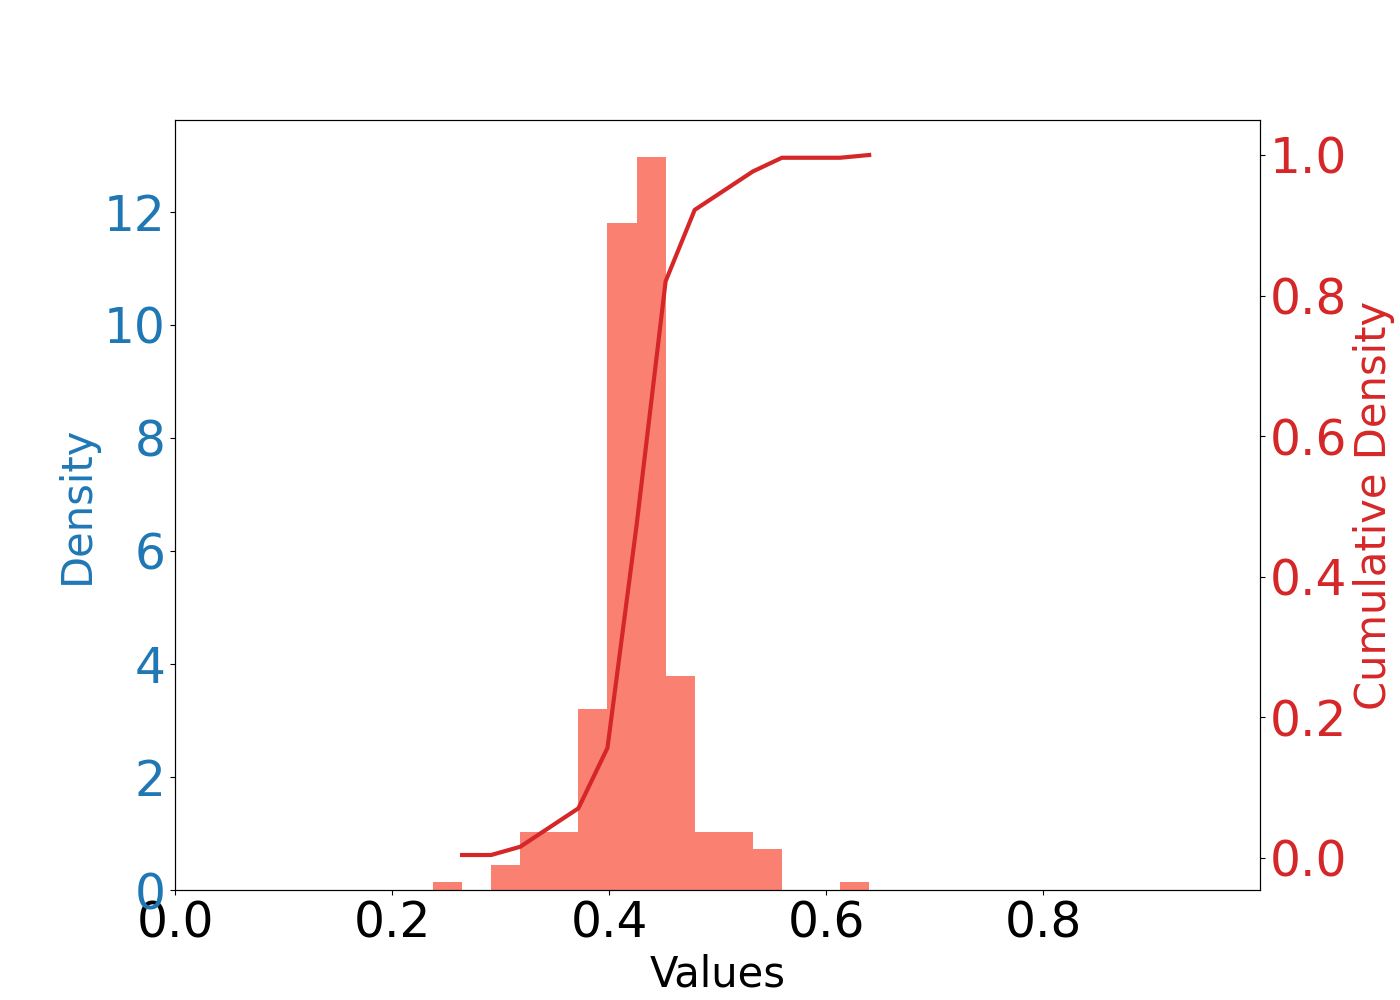
\includegraphics[scale=0.08]{figures/shot_density_idx_0_XCoord:9.24_YCoord:19.87.png}
    \end{minipage}
    \begin{minipage}{0.195\textwidth}
    \centering
    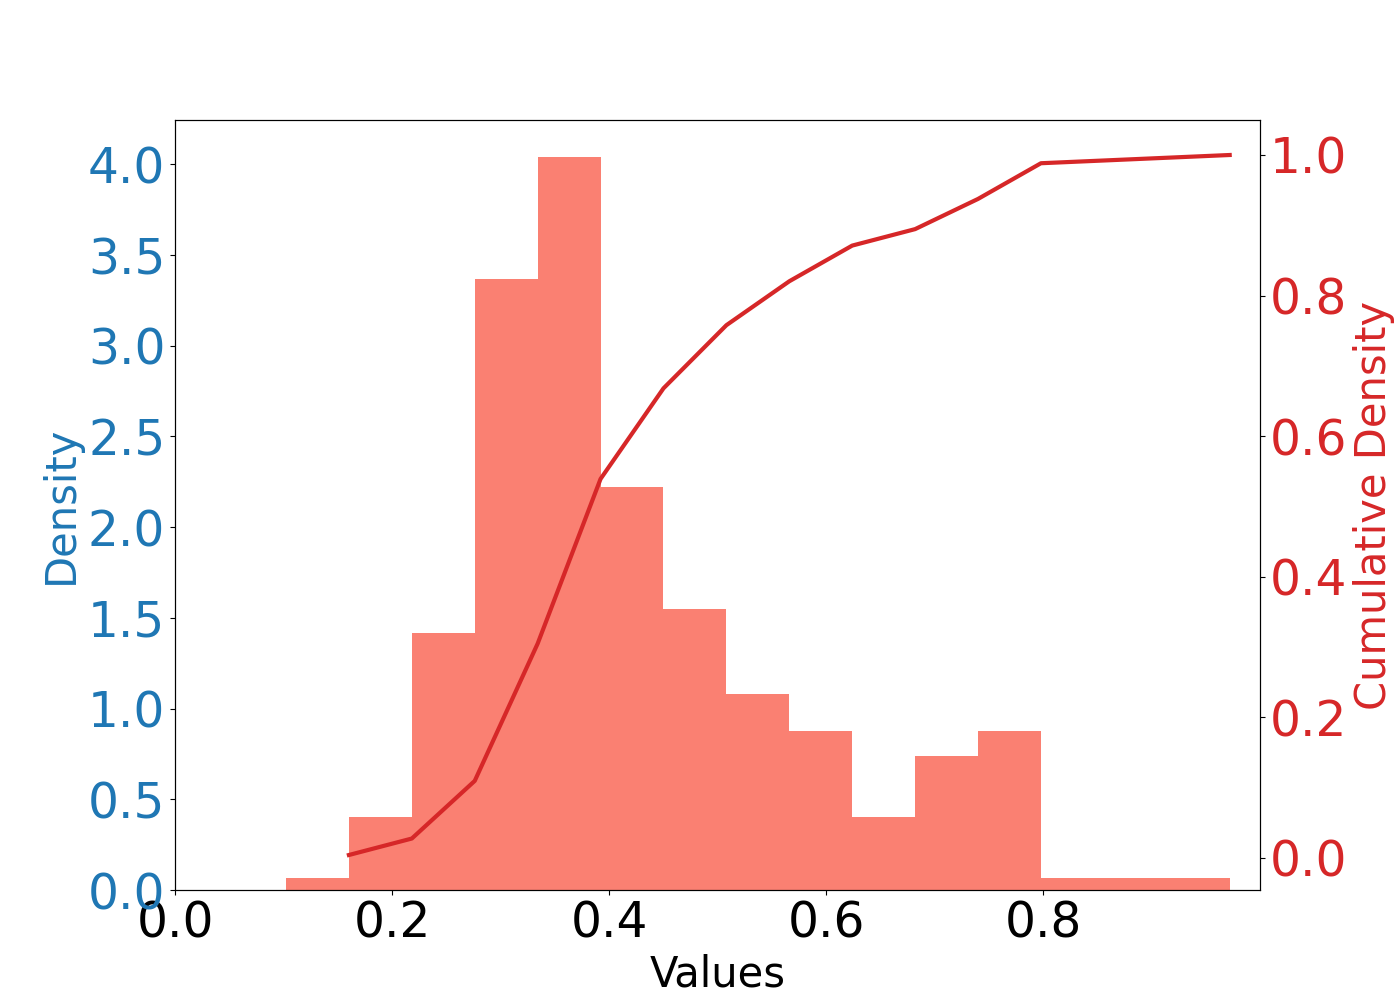
\includegraphics[scale=0.08]{figures/shot_density_idx_16_XCoord:79.27_YCoord:5.78.png}
    \end{minipage}
    \begin{minipage}{0.195\textwidth}
    \centering
    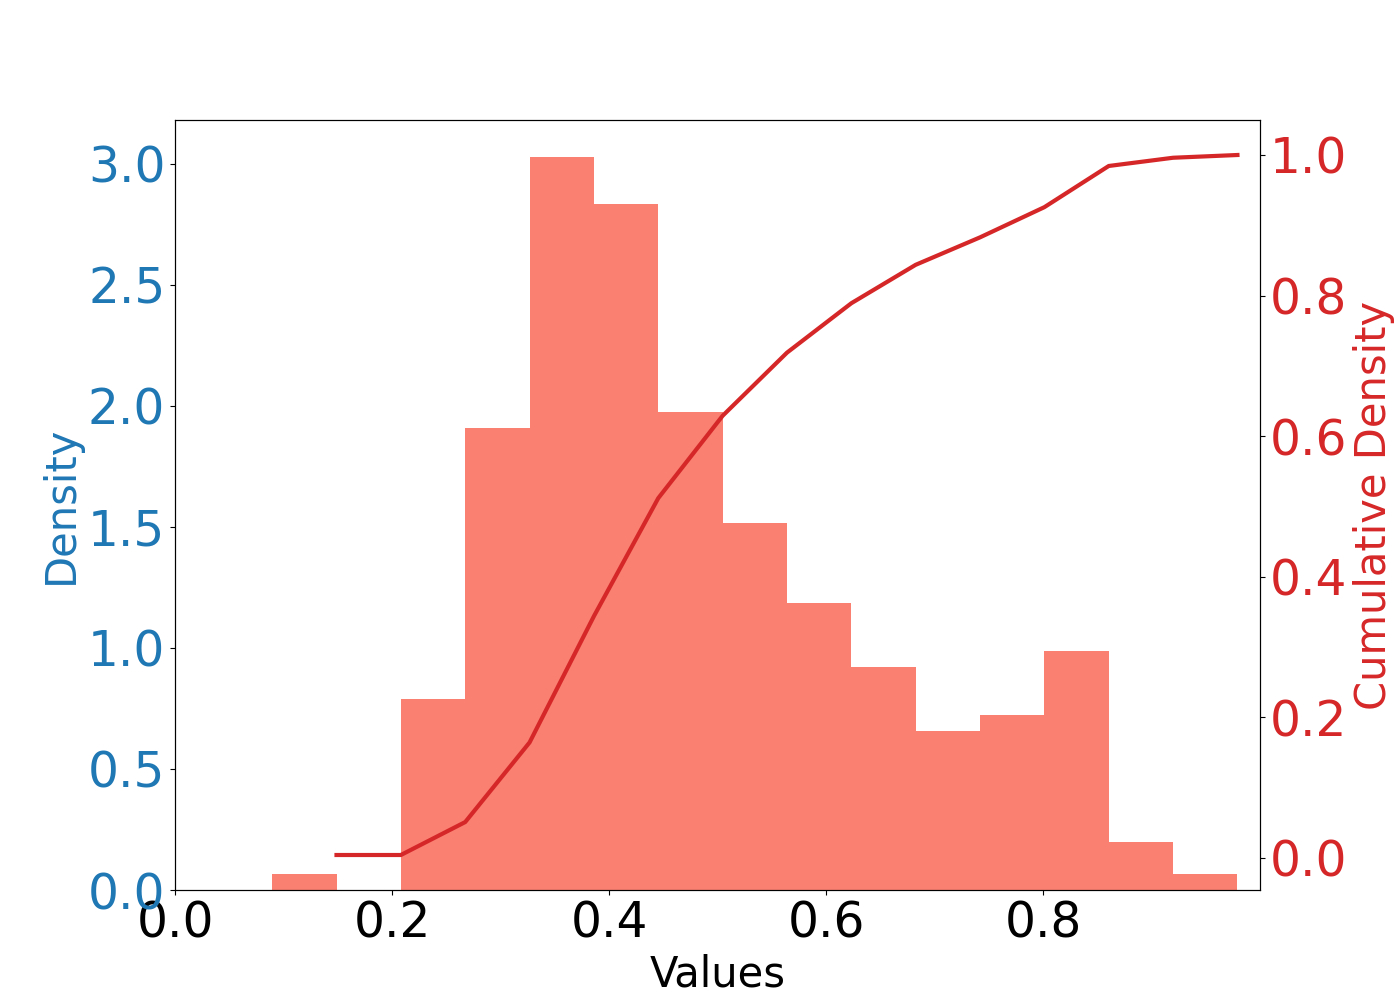
\includegraphics[scale=0.08]{figures/shot_density_idx_21_XCoord:74.75_YCoord:-0.25.png}
    \end{minipage}
    \begin{minipage}{0.195\textwidth}
    \centering
    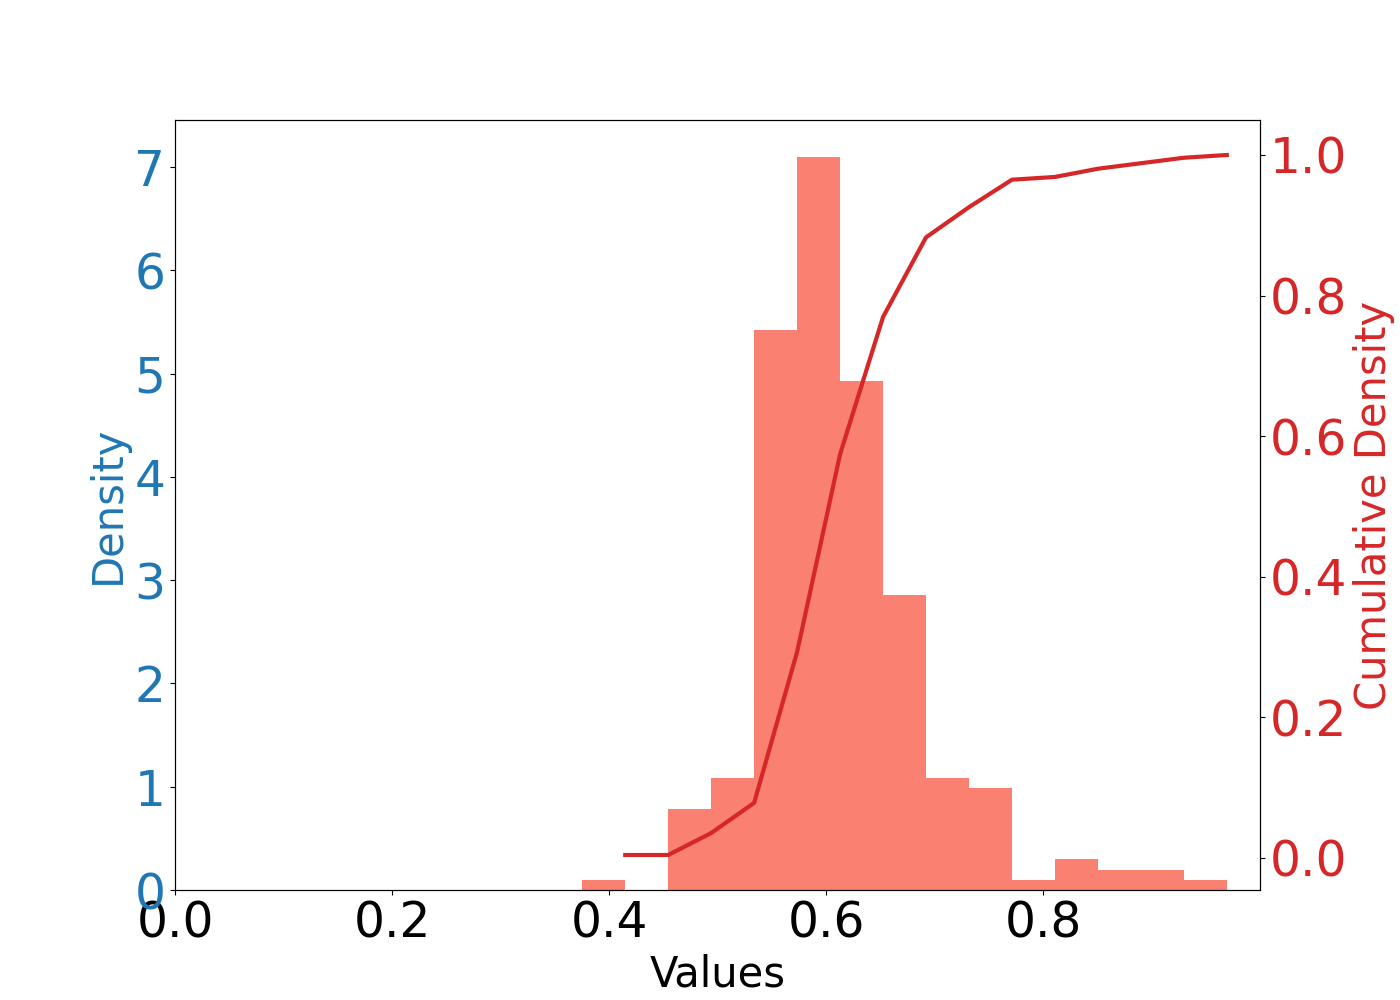
\includegraphics[scale=0.08]{figures/shot_density_idx_7_XCoord:85.69_YCoord:-21.88.png}
    \end{minipage}
    \begin{minipage}{0.195\textwidth}
    \centering
    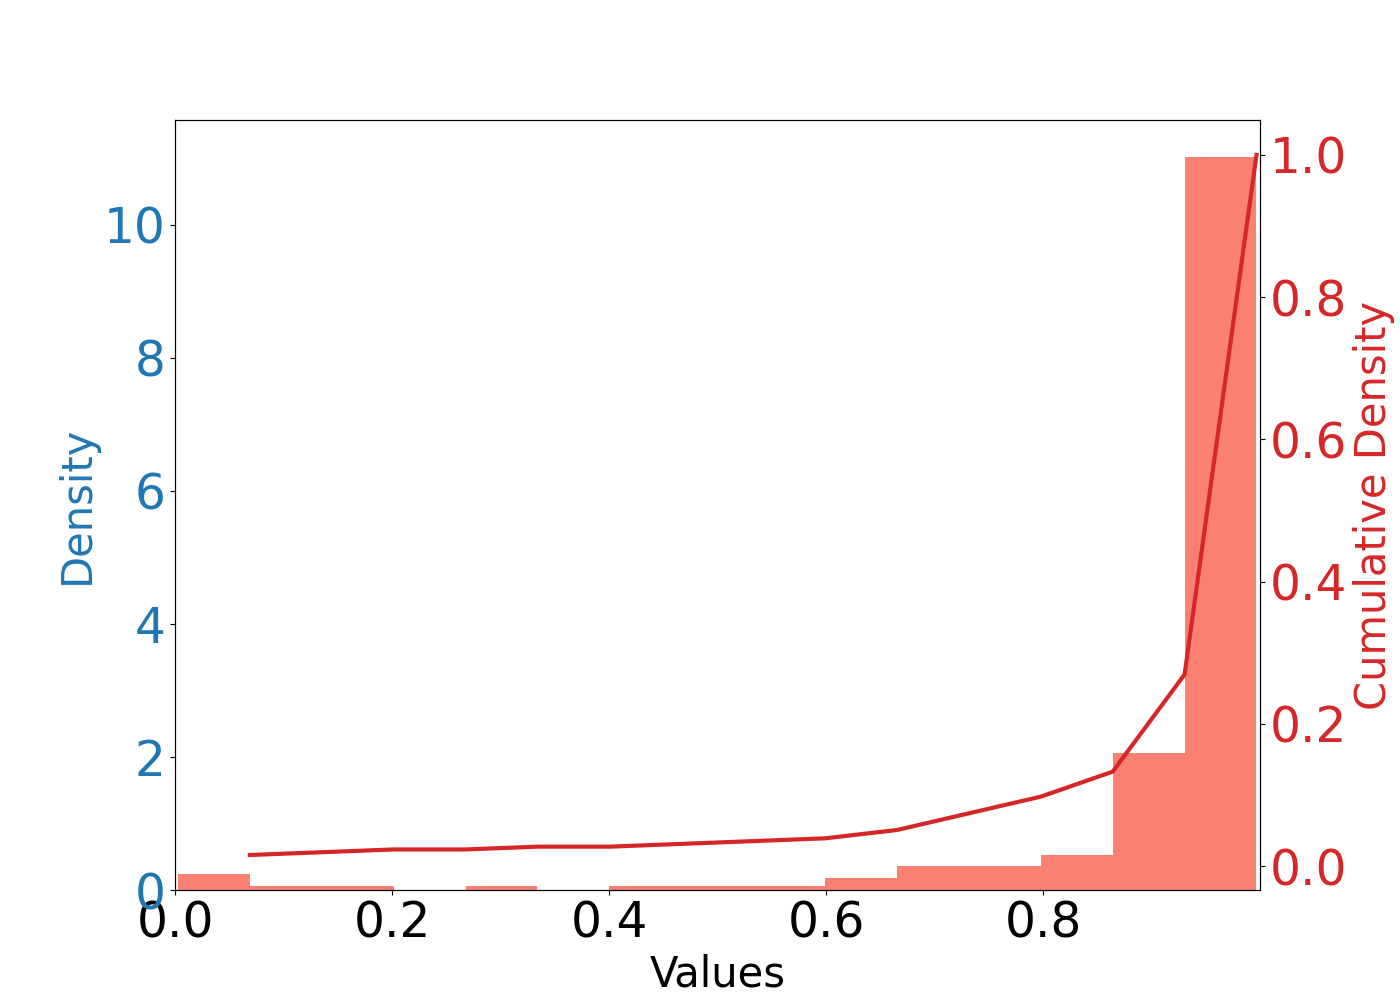
\includegraphics[scale=0.08]{figures/shot_density_idx_35_XCoord:-56.64_YCoord:-7.79.png}
    \end{minipage}
    \begin{minipage}{0.195\textwidth}
    \centering
    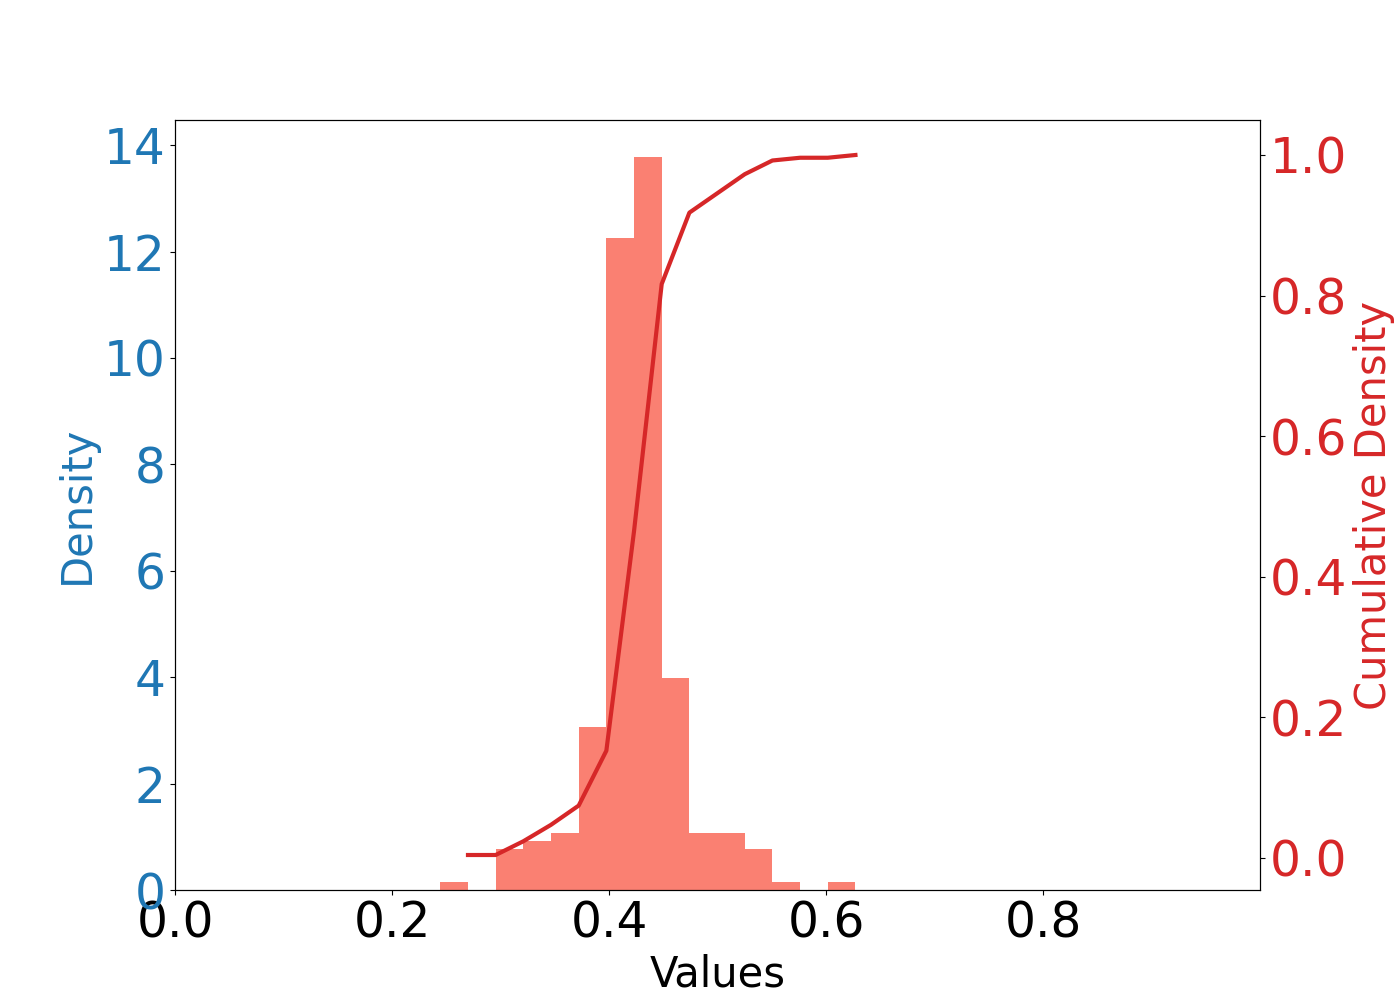
\includegraphics[scale=0.08]{figures/carry_density_idx_0_XCoord:0.19_YCoord:-38.47.png}
    \end{minipage}
    \begin{minipage}{0.195\textwidth}
    \centering
    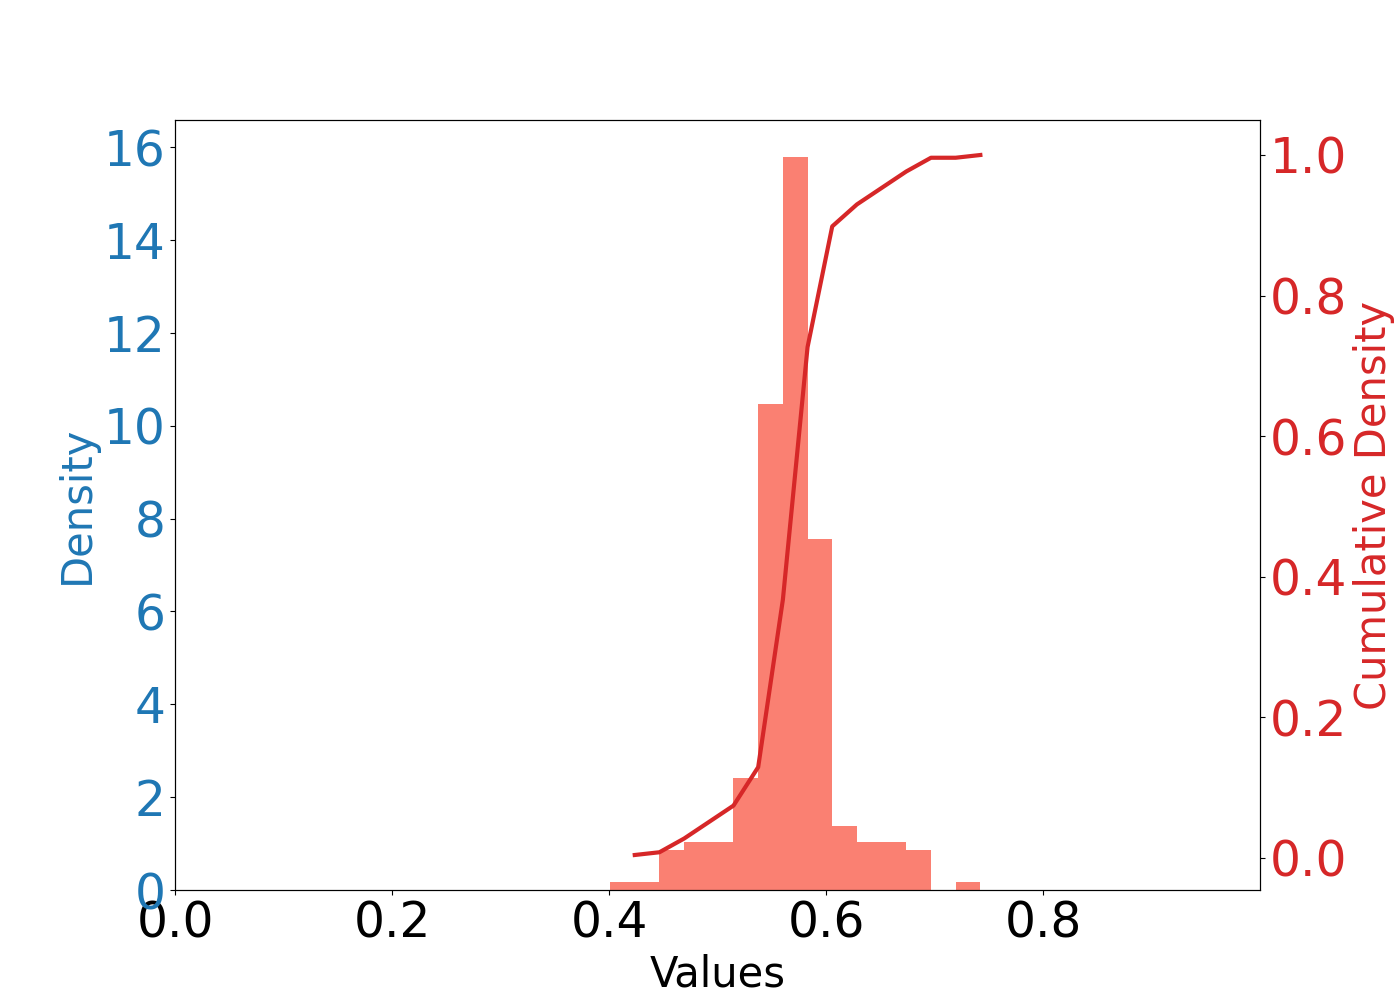
\includegraphics[scale=0.08]{figures/carry_density_idx_24_XCoord:-25.46_YCoord:-10.31.png}
    \end{minipage}
    \begin{minipage}{0.195\textwidth}
    \centering
    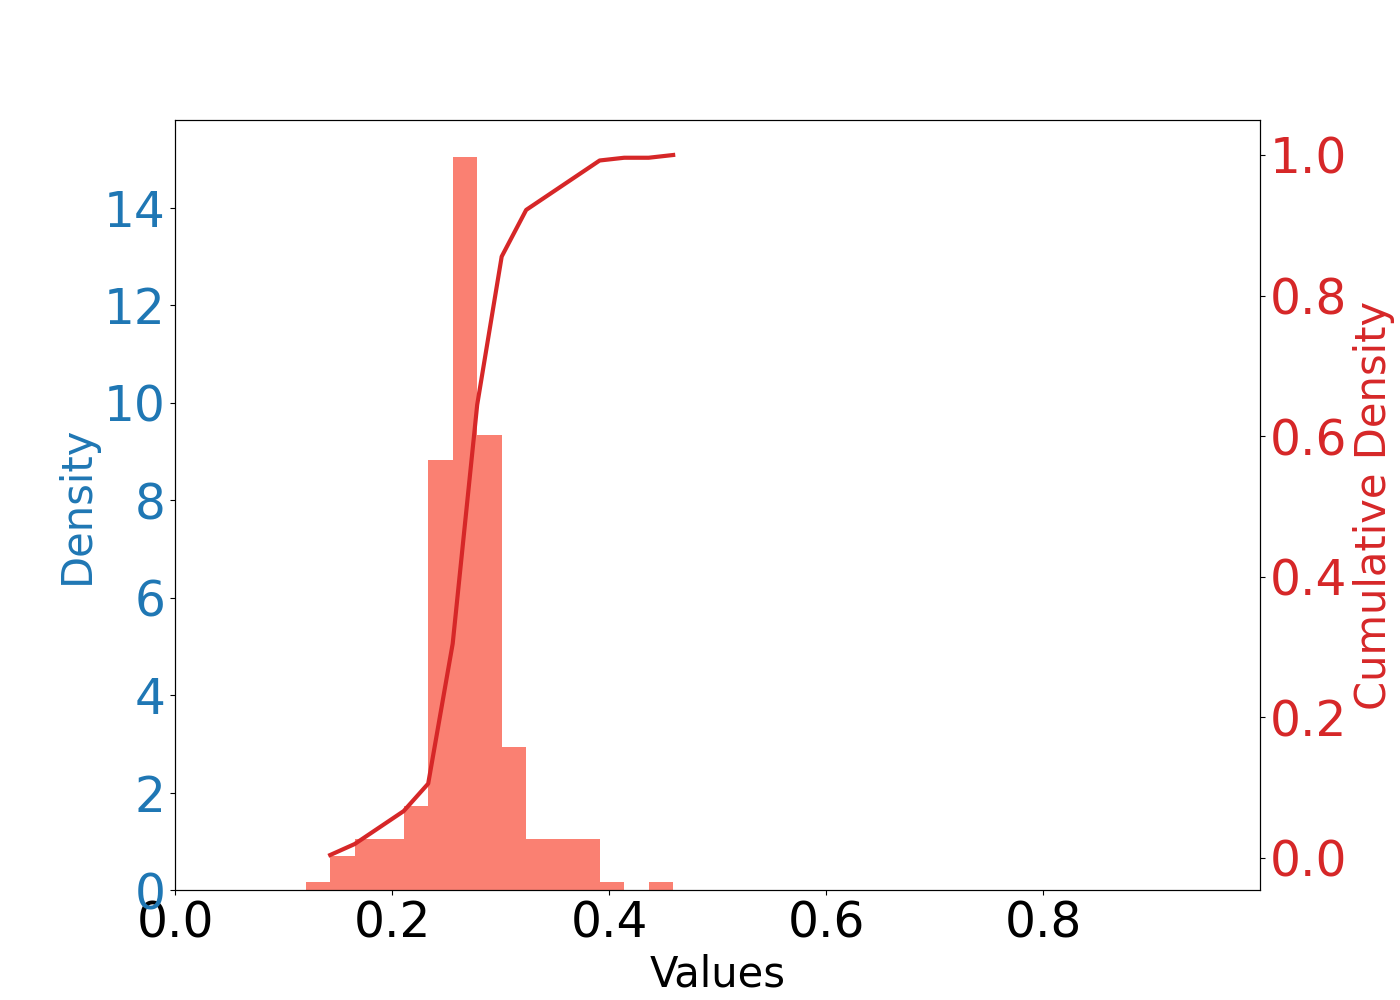
\includegraphics[scale=0.08]{figures/carry_density_idx_42_XCoord:0.31_YCoord:38.98.png}
    \end{minipage}
    \begin{minipage}{0.195\textwidth}
    \centering
    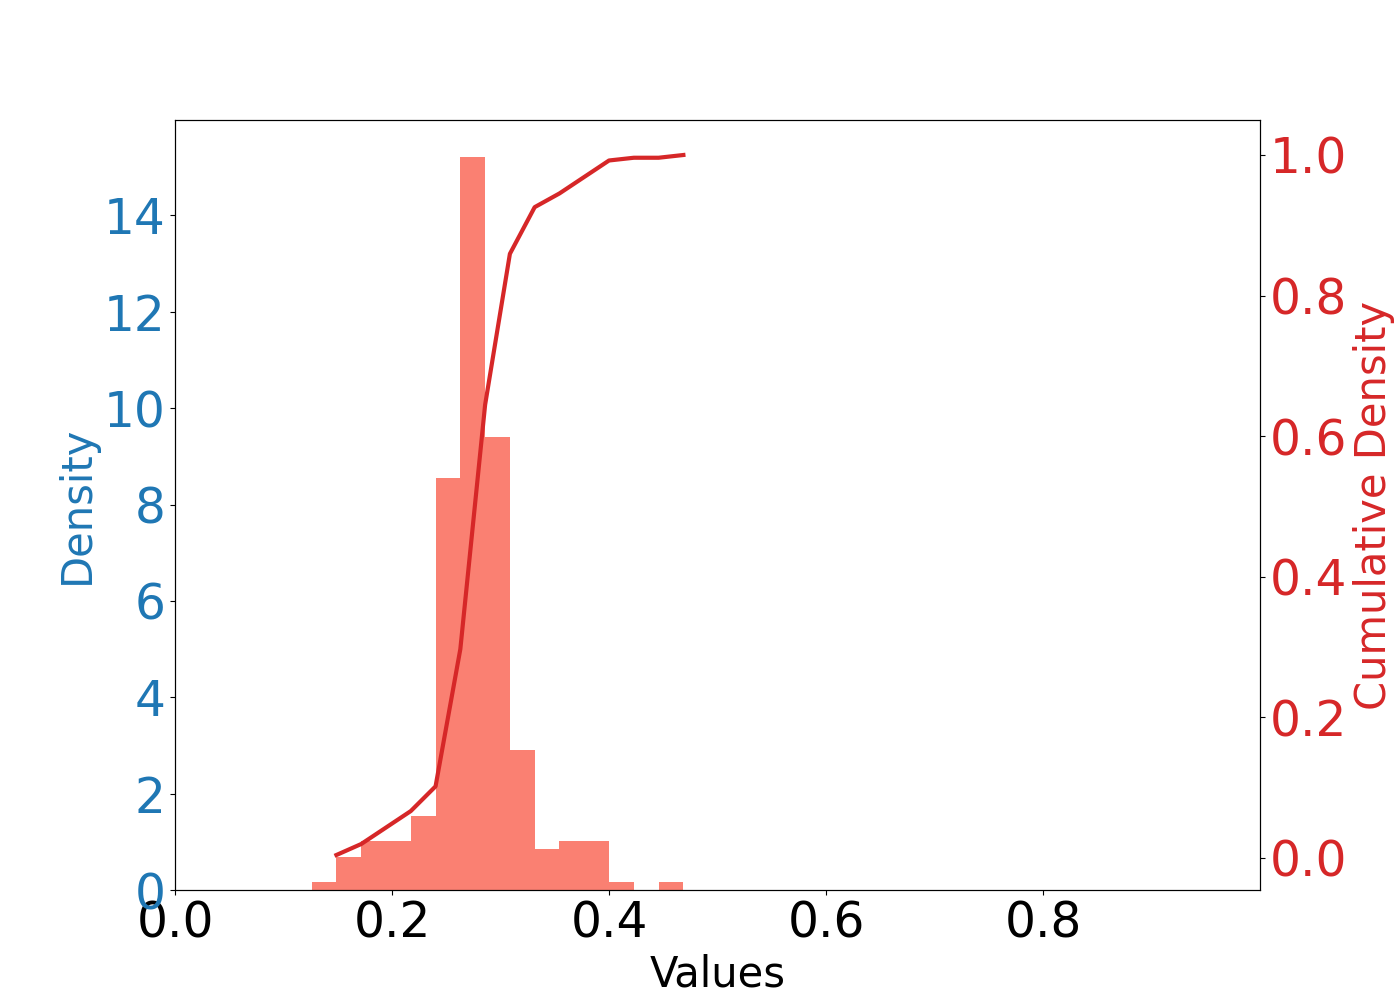
\includegraphics[scale=0.08]{figures/carry_density_idx_60_XCoord:-25.34_YCoord:12.82.png}
    \end{minipage}
    \begin{minipage}{0.195\textwidth}
    \centering
    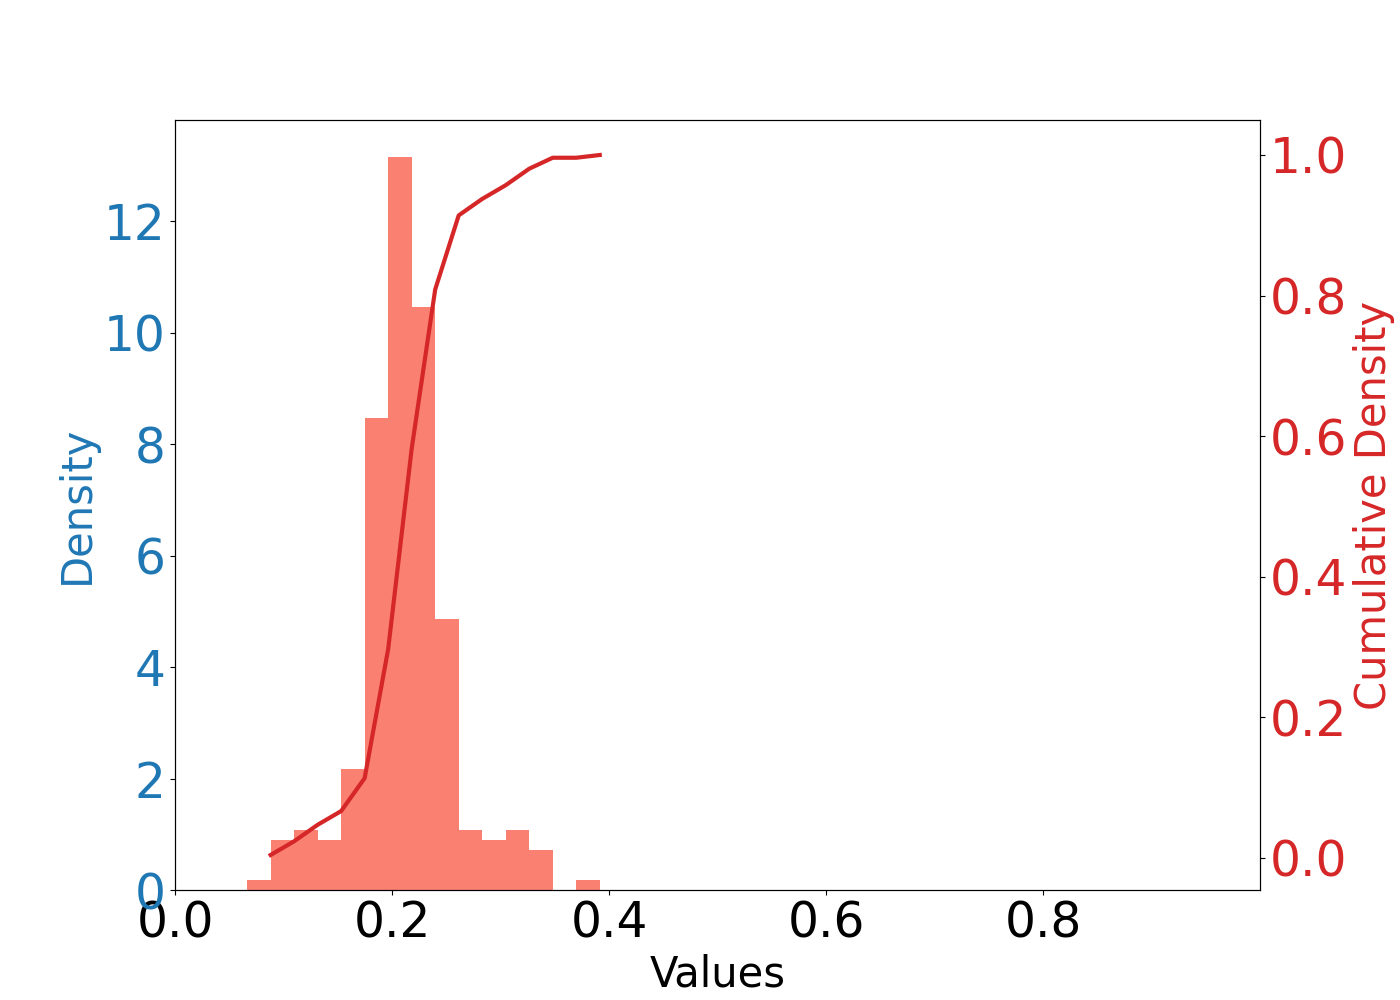
\includegraphics[scale=0.08]{figures/carry_density_idx_80_XCoord:0.19_YCoord:2.26.png}
    \end{minipage}
    \begin{minipage}{0.195\textwidth}
    \centering
    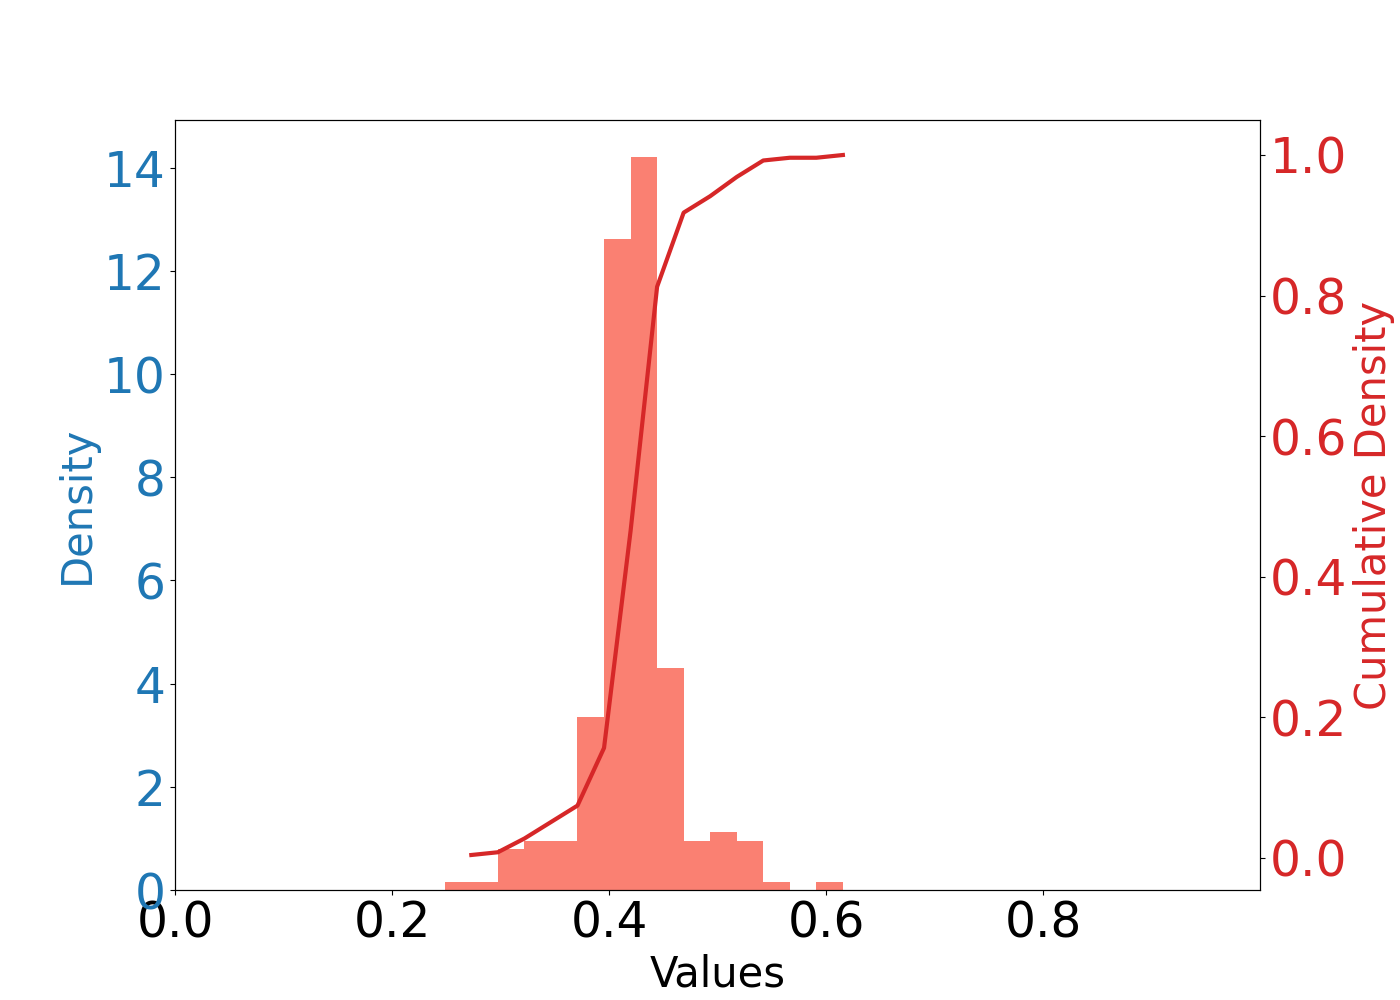
\includegraphics[scale=0.08]{figures/pass_density_idx_0_XCoord:-98.89_YCoord:13.33.png}
    \end{minipage}
    \begin{minipage}{0.195\textwidth}
    \centering
    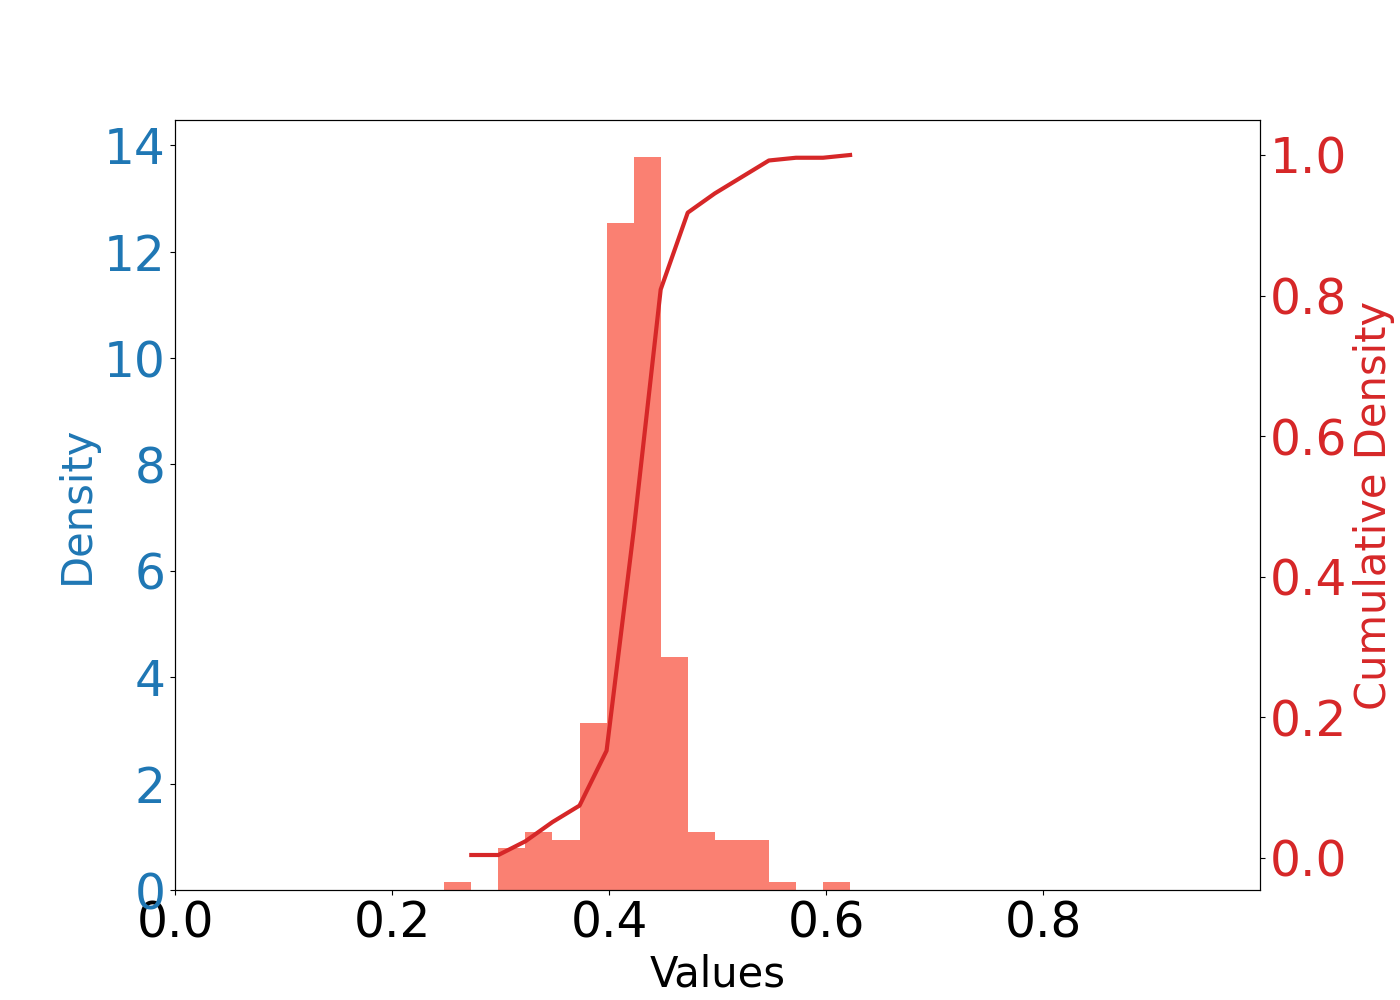
\includegraphics[scale=0.08]{figures/pass_density_idx_120_XCoord:81.16_YCoord:37.97.png}
    \end{minipage}
    \begin{minipage}{0.195\textwidth}
    \centering
    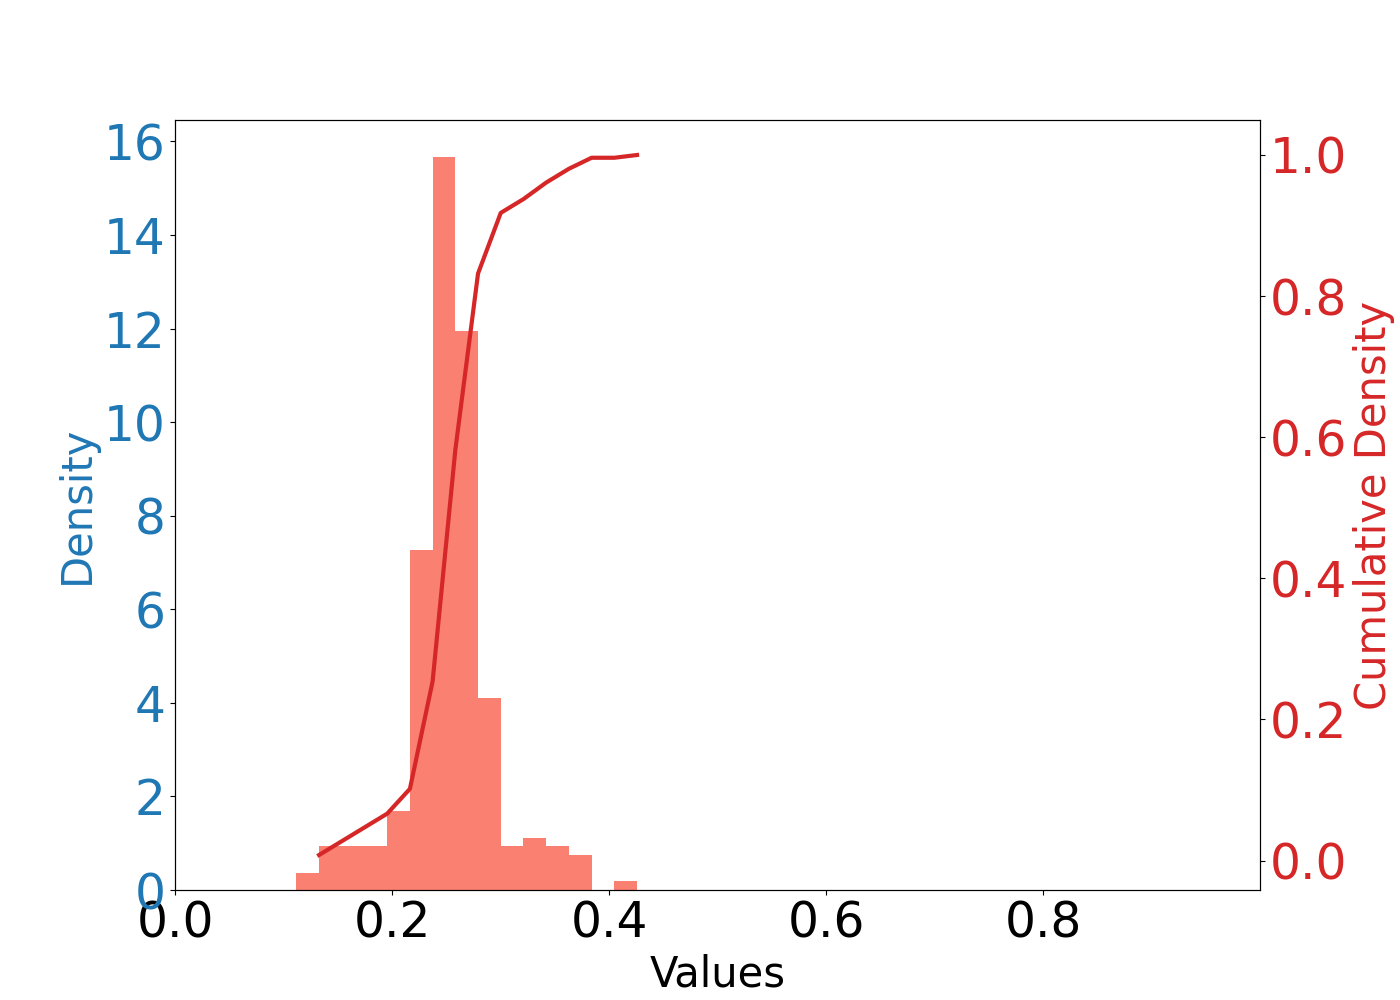
\includegraphics[scale=0.08]{figures/pass_density_idx_150_XCoord:-91.73_YCoord:7.29.png}
    \end{minipage}
    \begin{minipage}{0.195\textwidth}
    \centering
    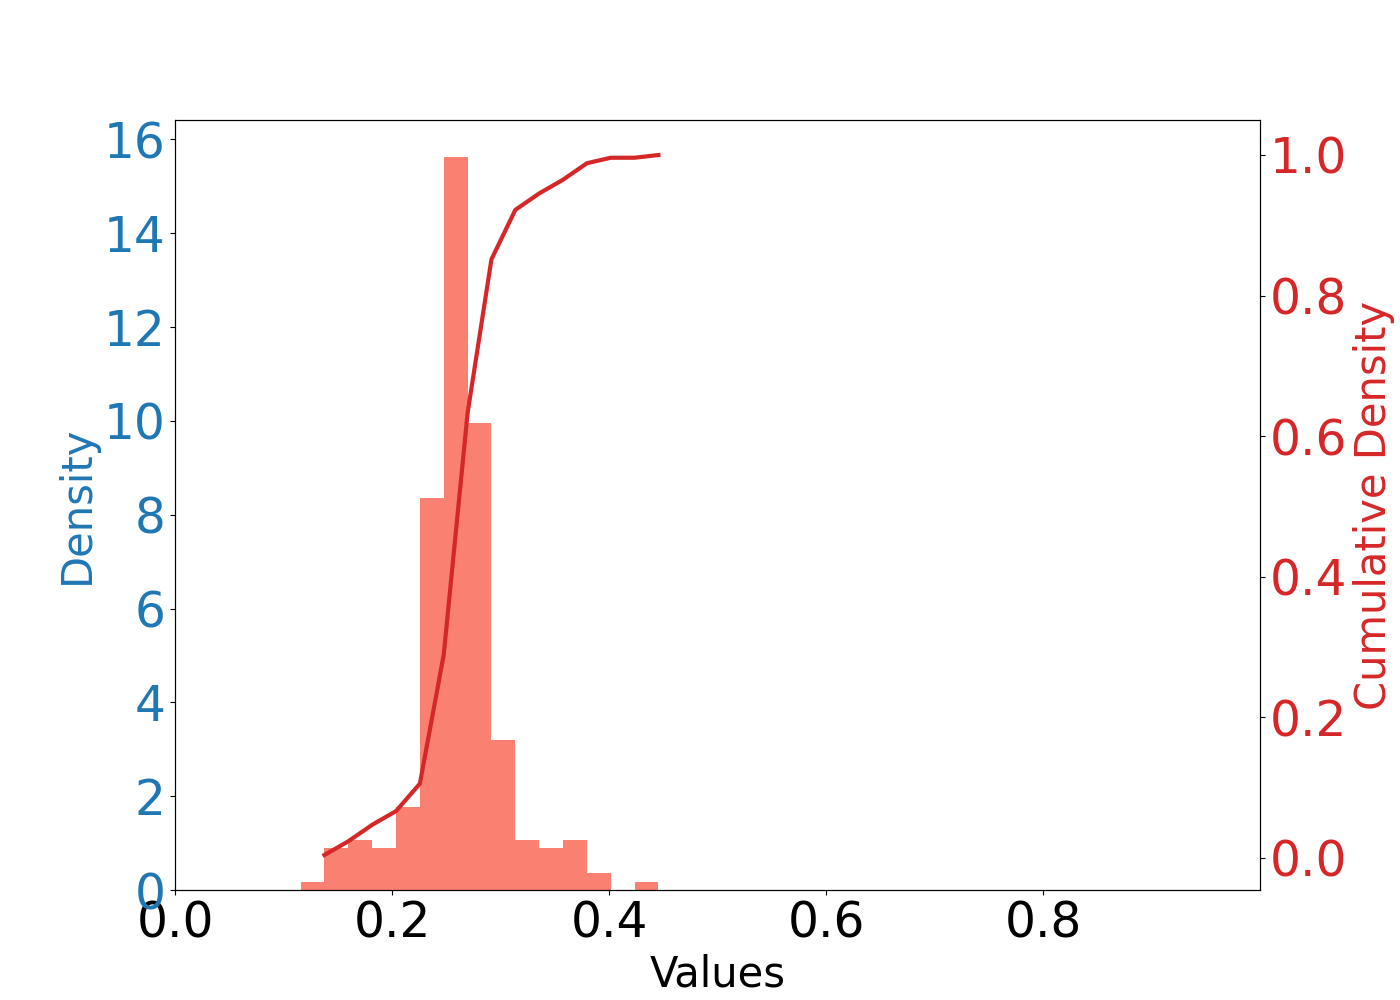
\includegraphics[scale=0.08]{figures/pass_density_idx_180_XCoord:-72.11_YCoord:0.75.png}
    \end{minipage}
    \begin{minipage}{0.195\textwidth}
    \centering
    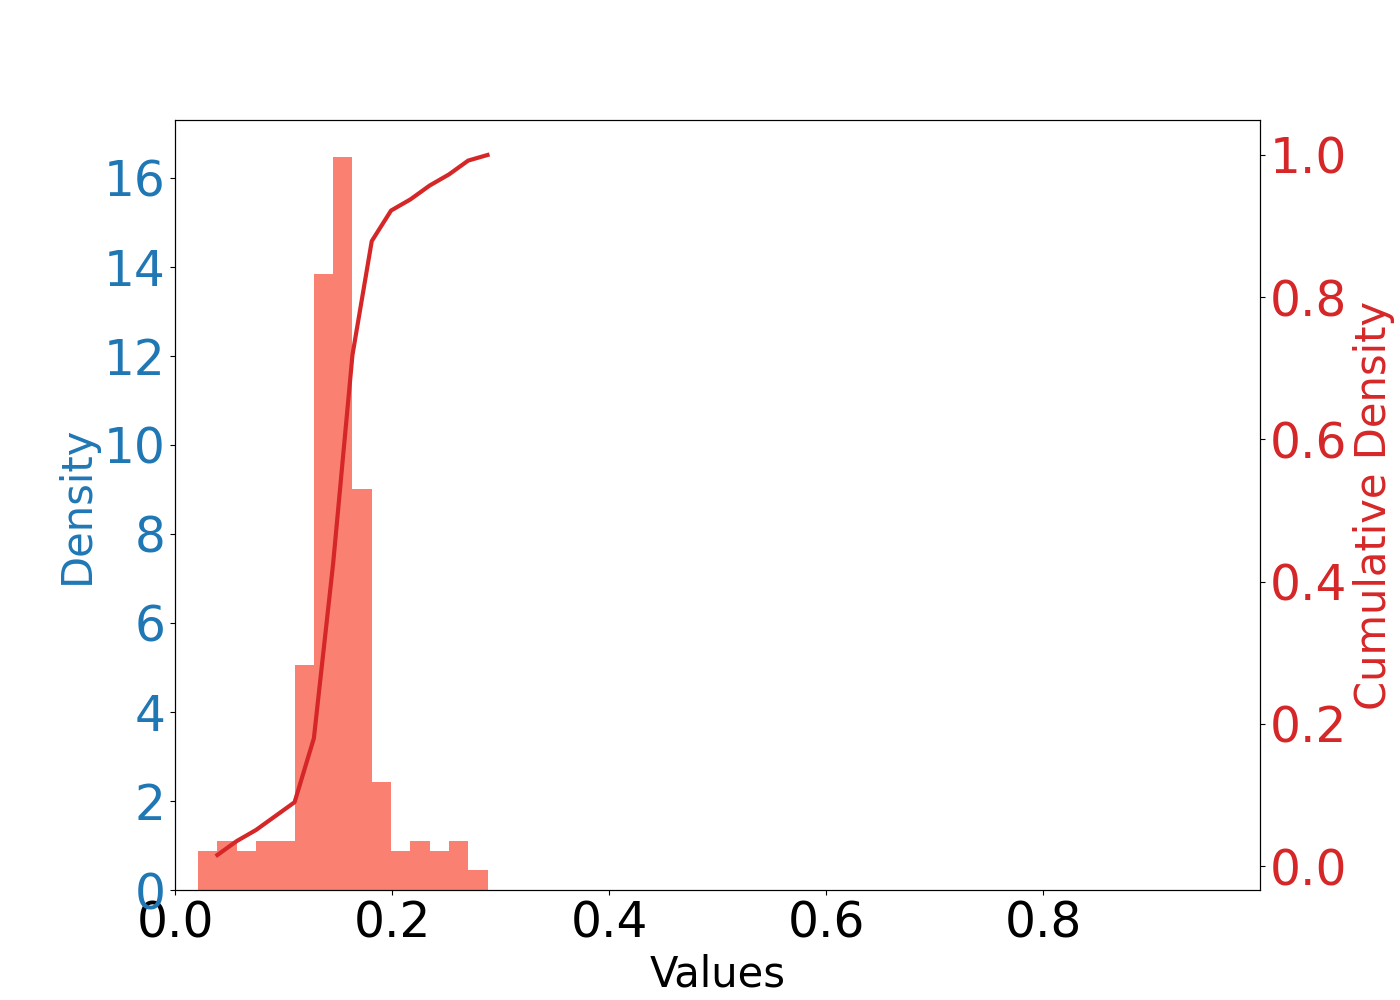
\includegraphics[scale=0.08]{figures/pass_density_idx_255_XCoord:-96.37_YCoord:-6.29.png}
    \end{minipage}
    \caption{Visualization of action-value distributions. From top to bottom, the actions are shot (top row), carry (middle row) and pass (bottom row). We show the 5 samples for each action.}~\label{fig:predicted-distribution-ice-hockey}
\end{figure*}

\subsection{The Scale of Uncertainty during Training}

We measure the epistemic uncertainty by the feature-space density estimator. In this section, we compute the scale of the density of the testing game as more games are observed during training. Figure~\ref{fig:uncertainty-by-games} shows the scale of epistemic uncertainty after training the model with different numbers of games. We find the scale of epistemic uncertainty decreases as more games are observed, which shows the model becomes more confident about its predictions after observing richer training data. This is a shred of evidence that data plays an important role in supporting decision-making. This result is consistent with the findings in~\cite{Mavrin2019DistributionalRL}.

\begin{figure}[htbp]
\begin{minipage}[t]{0.50\textwidth}
    \hspace{-0.25in}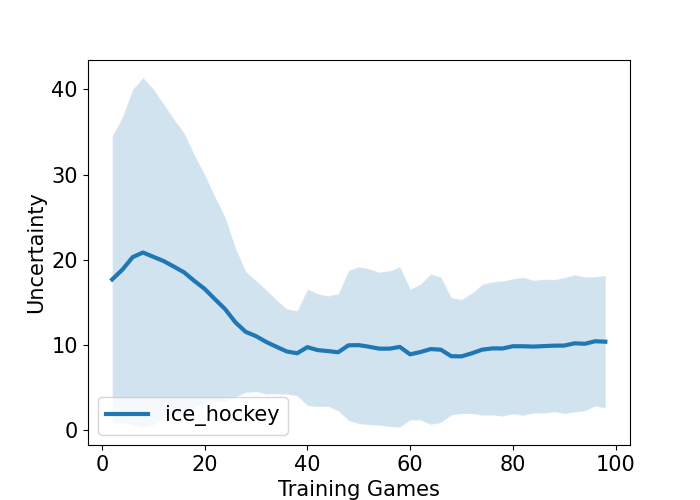
\includegraphics[scale=0.45]{figures/uncertainty_by_games_ice-hockey_maf_type-maf-split_blocks-5_inputs-45_hidden-180_cond-3_lr-0.0001_condValue_Aug-07-2022-23:50_shadow.png}
    \captionsetup{width=.95\linewidth}
\end{minipage}%
\begin{minipage}[t]{0.50\textwidth}
    \centering
    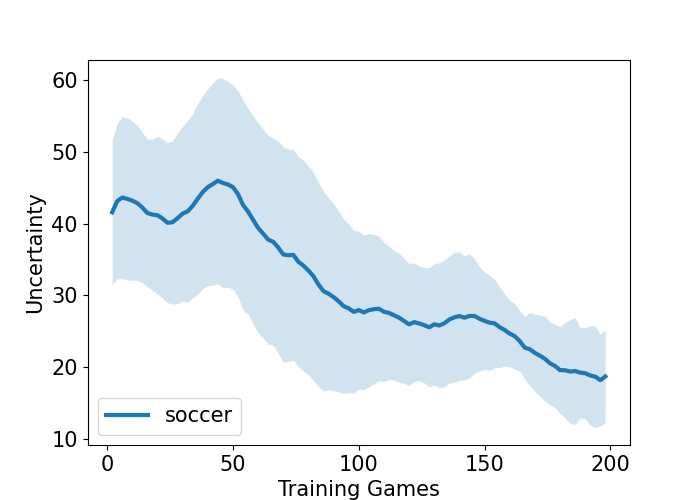
\includegraphics[scale=0.45]{figures/uncertainty_by_games_soccer_maf_type-maf-split_blocks-5_inputs-18_hidden-64_cond-46_lr-0.0001_condAct_condValue_Aug-08-2022-18:09_shadow.png}
    \captionsetup{width=.95\linewidth}
\end{minipage}
\caption{Illustrating the scale of epistemic uncertainty after observing more training games. The uncertainty is measured by the negative log-likelihood $-\log p(\state,\action|z)$ based on the outputs from the feature-space density estimator. We show the mean$\pm$std uncertainty computed with the games in the testing dataset.}
\label{fig:uncertainty-by-games}
\end{figure}

\subsection{Illustration of Temporal Projection} Figure~\ref{fig:temporal-plot} illustrates the mean $\pm$ standard deviation of the action-values sampled from the predicted distributions $\hat{Z}(\state,\action)$, where $\state$ and $\action$ follow the players' movements in a match between the Flyers (Home team) and the Maple Leafs (Away team) on March 15, 2019. The figure plots values
of the two output nodes. We highlight critical events and
match contexts to show the context-sensitivity of our predictions. 
\begin{figure}[htbp]
% \vspace{-0.2in}
    \centering
    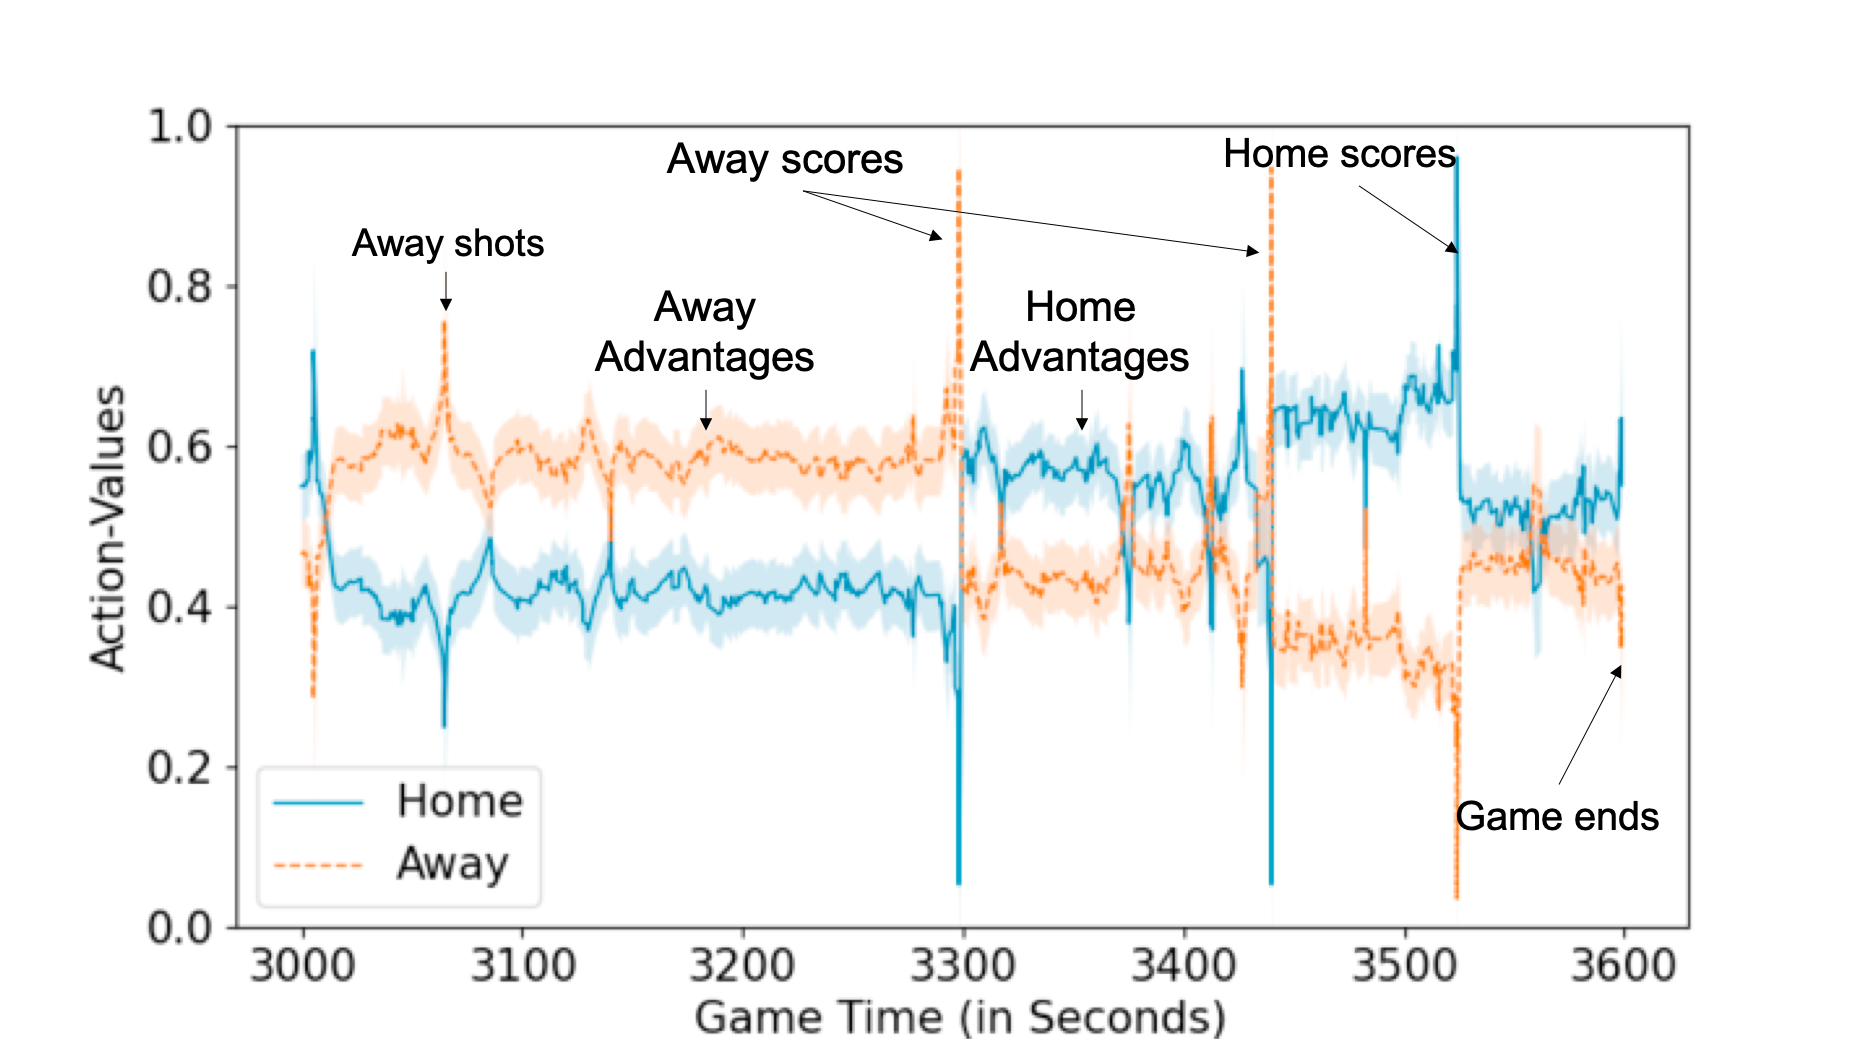
\includegraphics[scale=0.4]{figures/temporal-visualization-marked.png}
    % \captionsetup{width=.95\linewidth}
    \caption{Illustrating the predicted distributions by the mean $\pm$ standard deviation at each time step in a sports game.}~\label{fig:temporal-plot}
    % \vspace{-0.2in}
\end{figure}

Table~\ref{table:calibration-results} shows the complete (mean $\pm$ std) results in our scoring chance prediction experiment.

\begin{table}[htbp]
\centering
% \vspace{-0.15in}
\caption{The difference between the empirical and the estimated scoring chances in different contexts. Results are averaged over 5 runs $\pm$ standard error.  $\uparrow (\downarrow)$ indicates that a difference is statistically greater (smaller) than the difference achieved by \system with p-value $\le 0.01$ according to the Wilcoxon signed rank test.  }
\label{table:calibration-results}
\resizebox{1\textwidth}{!}{
\begin{tabular}{l|ccc:ccc}
\toprule
&\multicolumn{3}{c:}{Ice-Hockey} & \multicolumn{3}{c}{Soccer} \\\hline\hline
\begin{tabular}[c]{@{}c@{}}Manpower\\ Differential\end{tabular}& \begin{tabular}[c]{@{}c@{}}Short-\\ Handed\end{tabular} & \begin{tabular}[c]{@{}c@{}}Even-\\ Strength\end{tabular} & \begin{tabular}[c]{@{}c@{}}Power-\\ Play\end{tabular} & \begin{tabular}[c]{@{}c@{}}Short-\\ Handed\end{tabular} & \begin{tabular}[c]{@{}c@{}}Even-\\ Strength\end{tabular} & \begin{tabular}[c]{@{}c@{}}Power-\\ Play\end{tabular}\\\hline
GIM & 0.115 $\pm$ 0.078 $\downarrow$ & 0.094 $\pm$ 0.082 $\downarrow$ & 0.099 $\pm$ 0.085 $\downarrow$ & 0.211 $\pm$ 0.034 $\downarrow$ & {\bf 0.114} $\pm$ 0.05 $\uparrow$ & 0.199 $\pm$ 0.037 $\downarrow$ \\
Na-RiGIM & 0.133 $\pm$ 0.016 $\downarrow$ & 0.064 $\pm$ 0.016  $\downarrow$ & {\bf 0.013} $\pm$ 0.009 $\uparrow$ & 0.226 $\pm$ 0.019 $\downarrow$ & 0.136 $\pm$ 0.019  & 0.175 $\pm$ 0.028 $\downarrow$ \\
GDA-RiGIM & 0.148 $\pm$ 0.035 $\downarrow$ & 0.072 $\pm$ 0.029 $\downarrow$ & 0.017 $\pm$ 0.011  $\uparrow$ & 0.216 $\pm$ 0.022 $\downarrow$ & 0.151 $\pm$ 0.011 $\downarrow$ & 0.18 $\pm$ 0.013 $\downarrow$ \\
RiGIM & {\bf 0.080} $\pm$ 0.020 & {\bf 0.058} $\pm$ 0.008 & 0.047 $\pm$ 0.046 & {\bf 0.204} $\pm$ 0.005 & 0.133 $\pm$ 0.007 & {\bf 0.147} $\pm$ 0.033\\ \hline\hline
 Goal Differential & -1 & 0 & 1 & -1 & 0 & 1 \\\hline
GIM  & 0.238 $\pm$ 0.122 $\downarrow$ & 0.105 $\pm$ 0.084 $\downarrow$ & 0.271 $\pm$ 0.059 $\downarrow$ & 0.155 $\pm$ 0.047 $\downarrow$ & 0.155 $\pm$ 0.054 $\downarrow$ & 0.221 $\pm$ 0.049 $\downarrow$ \\
Na-RiGIM  & 0.238 $\pm$ 0.006 $\downarrow$ & 0.045 $\pm$ 0.015 $\downarrow$ & 0.108 $\pm$ 0.031 $\downarrow$ & 0.157 $\pm$ 0.02 & {\bf 0.104} $\pm$ 0.024 & 0.16 $\pm$ 0.017 $\downarrow$\\
GDA-RiGIM & 0.236 $\pm$ 0.007 $\downarrow$ & 0.045 $\pm$ 0.016 $\downarrow$ & 0.11 $\pm$ 0.027 & 0.165 $\pm$ 0.018 $\downarrow$ & 0.117 $\pm$ 0.017 $\downarrow$ & 0.175 $\pm$ 0.007 $\downarrow$\\
RiGIM & {\bf 0.193} $\pm$ 0.021 & {\bf 0.029} $\pm$ 0.015 & {\bf 0.092} $\pm$ 0.019 & {\bf 0.152} $\pm$ 0.008 & 0.109 $\pm$ 0.004 & {\bf 0.149} $\pm$ 0.013\\ \hline\hline
Period & 3 & 2 & 1 & 2$^{st}$ half
& 1$^{nd}$ half & N/A \\\hline
GIM & {\bf 0.095} $\pm$ 0.055 $\uparrow$ & 0.111 $\pm$ 0.086 $\downarrow$ & 0.114 $\pm$ 0.084 $\downarrow$ & {\bf 0.191} $\pm$ 0.037 $\uparrow$ & 0.104 $\pm$ 0.059 $\downarrow$ \\
Na-RiGIM  & 0.139 $\pm$ 0.018 & 0.044 $\pm$ 0.015 $\downarrow$ & 0.024 $\pm$ 0.015 $\downarrow$ & 0.237 $\pm$ 0.013 $\downarrow$ & 0.061 $\pm$ 0.03 $\downarrow$ \\
GDA-RiGIM & 0.143 $\pm$ 0.028 & 0.050 $\pm$ 0.025 $\downarrow$ & 0.033 $\pm$ 0.025 $\downarrow$ & 0.238 $\pm$ 0.012 $\downarrow$ & 0.059 $\pm$ 0.026\\
RiGIM & 0.143 $\pm$ 0.011 & {\bf 0.032} $\pm$ 0.005 & {\bf 0.014} $\pm$ 0.009  & 0.226 $\pm$ 0.011 & {\bf 0.058} $\pm$ 0.009\\ \bottomrule
\end{tabular}
}
\end{table}


\section{Negative Social Impact}
We expect the main impact outside of the machine learning community to be in professional sports. As part of the entertainment industry, professional sports increase the quality of life for many people. Fans, media, and clubs can be better engaged in sports games with a player ranking system, but putting players’ performance under intense scrutiny may yield more pressure on the professional players. The overwhelming pressure might cause anxiety and thus contradicts the original purpose of evaluating players, which is about improving their playing skills and market value.

% \newpage

% \subsection{Proof 2}
% \begin{align*}
%     & Var(Z(\state,\action|\dataset))\\
%     &\stackrel{\mathclap{\normalfont\mbox{(a)}}}{=}Var(R(s,a)+\gamma P^{\pi}Z({\state}^{\prime},{\action}^{\prime})|\dataset) \\
%     &\stackrel{\mathclap{\normalfont\mbox{(b)}}}{=}H(\MakeUppercase{\state}^{\prime}|\MakeUppercase{\state}=\state,\MakeUppercase{\action}=\action) + H(\MakeUppercase{\action}^{\prime}|\MakeUppercase{\state}^{\prime},\MakeUppercase{\state}=\state,\MakeUppercase{\action}=\action) + H(\MakeUppercase{Z}^{\prime}|\MakeUppercase{\state}^{\prime},\MakeUppercase{\action}^{\prime},\MakeUppercase{\state}=\state,\MakeUppercase{\action}=\action,\dataset)\\
% \end{align*}

% \newpage
% \subsection{Proof 3}
% \begin{align*}
%     & H(Z(\state,\action|\dataset))\\
%     &=H(Z|\MakeUppercase{\state}=\state,\MakeUppercase{\action}=\action,\dataset))\\
%     &\stackrel{\mathclap{\normalfont\mbox{(a)}}}{=}H(R(s,a)+\gamma P^{\pi}Z({\state}^{\prime},{\action}^{\prime})|\dataset) \\
%     &\stackrel{\mathclap{\normalfont\mbox{(b)}}}{=}H(\MakeUppercase{\state}^{\prime},\MakeUppercase{\action}^{\prime},\MakeUppercase{Z}^{\prime}|\dataset,\MakeUppercase{\state}=\state,\MakeUppercase{\action}=\action)\\
%     &\stackrel{\mathclap{\normalfont\mbox{(c)}}}{=}H(\MakeUppercase{\state}^{\prime}|\MakeUppercase{\state}=\state,\MakeUppercase{\action}=\action) + H(\MakeUppercase{\action}^{\prime}|\MakeUppercase{\state}^{\prime},\MakeUppercase{\state}=\state,\MakeUppercase{\action}=\action) + H(\MakeUppercase{Z}^{\prime}|\MakeUppercase{\state}^{\prime},\MakeUppercase{\action}^{\prime},\MakeUppercase{\state}=\state,\MakeUppercase{\action}=\action,\dataset)\\
%     % &\stackrel{\mathclap{\normalfont\mbox{(d)}}}{=}H(\MakeUppercase{\state}^{\prime}|\MakeUppercase{\state}=\state,\MakeUppercase{\action}=\action) + H(\MakeUppercase{\action}^{\prime}|\MakeUppercase{\state}^{\prime},\MakeUppercase{\state}=\state,\MakeUppercase{\action}=\action) + \sum_{\state^{\prime},\action^{\prime}} p(\state^{\prime},\action^{\prime}|\MakeUppercase{\state}=\state,\MakeUppercase{\action}=\action,\dataset) H(\MakeUppercase{Z}^{\prime}|\MakeUppercase{\state}^{\prime}=\state^{\prime},\MakeUppercase{\action}^{\prime}=\action^{\prime},\dataset) \mathrm{d}(\state^{\prime},\action^{\prime})\\
%     &\stackrel{\mathclap{\normalfont\mbox{(d)}}}{=}H(\MakeUppercase{\state}^{\prime}|\MakeUppercase{\state}=\state,\MakeUppercase{\action}=\action) + H(\MakeUppercase{\action}^{\prime}|\MakeUppercase{\state}^{\prime},\MakeUppercase{\state}=\state,\MakeUppercase{\action}=\action) + \sum_{\state^{\prime},\action^{\prime}} \rho^{\pi}(\state,\action\rightarrow\state^{\prime}\action^{\prime};1|\dataset) H(\MakeUppercase{Z}^{\prime}|\MakeUppercase{\state}^{\prime}=\state^{\prime},\MakeUppercase{\action}^{\prime}=\action^{\prime},\dataset)\\
%     &\stackrel{\mathclap{\normalfont\mbox{(e)}}}{=}H(\MakeUppercase{\state}^{\prime}|\MakeUppercase{\state}=\state,\MakeUppercase{\action}=\action) + H(\MakeUppercase{\action}^{\prime}|\MakeUppercase{\state}^{\prime},\MakeUppercase{\state}=\state,\MakeUppercase{\action}=\action) + \sum_{\state^{\prime},\action^{\prime}} \rho^{\pi}(\state,\action\rightarrow\state^{\prime}\action^{\prime};1|\dataset) \Big[H(\MakeUppercase{\state}^{\prime\prime}|\MakeUppercase{\state}^{\prime}=\state^{\prime},\MakeUppercase{\action}^{\prime}=\action^{\prime}) \\ 
%     & + H(\MakeUppercase{\action}^{\prime\prime}|\MakeUppercase{\state}^{\prime\prime},\MakeUppercase{\state}^{\prime}=\state^{\prime},\MakeUppercase{\action}^{\prime}=\action^{\prime}) + \sum_{\state^{\prime\prime},\action^{\prime\prime}} \rho^{\pi}(\state^{\prime},\action^{\prime}\rightarrow\state^{\prime\prime}\action^{\prime\prime};1|\dataset) H(\MakeUppercase{Z}^{\prime\prime}|\MakeUppercase{\state}^{\prime\prime}=\state^{\prime\prime},\MakeUppercase{\action}^{\prime\prime}=\action^{\prime\prime},\dataset)\Big]\\
%     &\stackrel{\mathclap{\normalfont\mbox{(f)}}}{=}\phi(\state,\action)+\sum_{\state^{\prime},\action^{\prime}}\rho^{\pi}(\state,\action\rightarrow\state^{\prime}\action^{\prime};1|\dataset)\phi(\state^{\prime},\action^{\prime})+\sum_{\state^{\prime\prime},\action^{\prime\prime}}\rho^{\pi}(\state,\action\rightarrow\state^{\prime\prime}\action^{\prime\prime};2|\dataset)H(Z^{\prime\prime}|\MakeUppercase{\state}^{\prime\prime}=\state^{\prime\prime},\MakeUppercase{\action}^{\prime\prime}=\action^{\prime\prime})\\
%     &\stackrel{\mathclap{\normalfont\mbox{(g)}}}{=}\sum_{\Tilde{\state},\Tilde{\action}}\sum_{k=0}^{\horizon-t}\rho^{\pi}(\state,\action\rightarrow\Tilde{\state},\Tilde{\action};k|\dataset)\phi(\Tilde{\state},\Tilde{\action})\\
%     &\stackrel{\mathclap{\normalfont\mbox{(h)}}}{=}\sum_{\Tilde{\state},\Tilde{\action}}\eta(\Tilde{\state},\Tilde{\action}|\dataset)\sum_{\Tilde{\state},\Tilde{\action}}\frac{\eta(\Tilde{\state},\Tilde{\action}|\dataset)}{\sum_{\Tilde{\state},\Tilde{\action}}\eta(\Tilde{\state},\Tilde{\action}|\dataset)}
%     \phi(\Tilde{\state},\Tilde{\action})\\
%     &\stackrel{\mathclap{\normalfont\mbox{(i)}}}{=}\constant\cdot\sum_{\Tilde{\state},\Tilde{\action}}d^{\pi}(\Tilde{\state},\Tilde{\action}|\dataset)\phi(\Tilde{\state},\Tilde{\action})
% \end{align*}
% % \textcolor{blue}{or we apply an empirical approximation to the integral here.}

% Where 
% \begin{itemize}
%     \item (a) holds since we assume the Bellman consistency.
%     \item (b) holds because 1) the dynamic matrix
%     \begin{align*}
%     P^{\pi}
%         & =\sum P^{\pi}_{(\state,\action),(\state^{\prime},\action^{\prime})} \mathrm{d}(\state^{\prime},\action^{\prime})\\
%         & =\sum P(\state^{\prime}|\state,\action) \pi(\action^{\prime}|\state^{\prime}) \mathrm{d}(\state^{\prime},\action^{\prime}) \\
%         & =\sum \pi(\action^{\prime}|\state^{\prime}) \mathrm{d}\action^{\prime} P(\state^{\prime}|\state,\action) \mathrm{d}\state^{\prime}
%     \end{align*}
%     2) adding a reward is equivalent to shift the distribution by $\MakeUppercase{\reward}(\state,\action)$, which does not influence the entropy of distribution. 3) we assume $\gamma=1$.
%     \item (c) holds because of 1) the Markov property in a MDP 2) the independence between the training dataset $\dataset$ and the transition and the policy functions 3) by the chain rules of conditional entropy by following the dependency $\MakeUppercase{\state}\longrightarrow\MakeUppercase{\action}\longrightarrow\MakeUppercase{\state}^{\prime}\longrightarrow\MakeUppercase{\action}^{\prime}$.
%     \item (d) holds following the definition of  conditional entropy and $\rho^{\pi}(\state,\action\rightarrow\state^{\prime}\action^{\prime};k|\dataset)$ denotes the estimation of the probability of transitioning from state-action pair $(\state,\action)$ to $(\state^{\prime},\action^{\prime})$ with policy $\pi$ after $k$ step.
%     \item (e) holds by substituting $H(\MakeUppercase{Z}^{\prime}|\MakeUppercase{\state}^{\prime}=\state^{\prime},\MakeUppercase{\action}^{\prime}=\action^{\prime},\dataset)$ with $H(\MakeUppercase{\state}^{\prime\prime}|\MakeUppercase{\state}^{\prime}=\state^{\prime},\MakeUppercase{\action}^{\prime}=\action^{\prime}) + H(\MakeUppercase{\action}^{\prime\prime}|\MakeUppercase{\state}^{\prime\prime},\MakeUppercase{\state}^{\prime}=\state^{\prime},\MakeUppercase{\action}^{\prime}=\action^{\prime}) + \sum_{\state^{\prime\prime},\action^{\prime\prime}} \rho^{\pi}(\state^{\prime},\action^{\prime}\rightarrow\state^{\prime\prime}\action^{\prime\prime};1|\dataset) H(\MakeUppercase{Z}^{\prime\prime}|\MakeUppercase{\state}^{\prime\prime}=\state^{\prime\prime},\MakeUppercase{\action}^{\prime\prime}=\action^{\prime\prime},\dataset) \mathrm{d}(\state^{\prime\prime},\action^{\prime\prime})$.
%     \item (f) holds because we let $\phi(\state,\action)=H(\MakeUppercase{\state}^{\prime}|\MakeUppercase{\state}=\state,\MakeUppercase{\action}=\action) + H(\MakeUppercase{\action}^{\prime}|\MakeUppercase{\state}^{\prime},\MakeUppercase{\state}=\state,\MakeUppercase{\action}=\action)$.
%     \item (g) holds.
%     \item (h) holds $\eta(\Tilde{\state},\Tilde{\action}|\dataset)=\sum_{k=0}^{T_{g}}\rho^{\pi}(\state,\action\rightarrow\Tilde{\state},\Tilde{\action};k|\dataset)$.
%     \item (i) holds because $d^{\pi}(\Tilde{\state},\Tilde{\action}|\dataset)=\frac{\eta(\Tilde{\state},\Tilde{\action}|\dataset)}{\sum_{\Tilde{\state},\Tilde{\action}}\eta(\Tilde{\state},\Tilde{\action}|\dataset)}$ and we represent the constant $\sum_{\Tilde{\state},\Tilde{\action}}\eta(\Tilde{\state},\Tilde{\action}|\dataset)$ with $\constant$. 
% \end{itemize}
\bibliographystyle{unsrt}
\bibliography{bibliography.bib}



\end{document}